% =====================================================================
%  Tomito-RS -- Visual Architecture Guide
%  Build: pdflatex architecture.tex  (twice, for the ToC)
% =====================================================================
\documentclass[11pt,a4paper]{article}

\usepackage[T1]{fontenc}
\usepackage[utf8]{inputenc}
\usepackage{lmodern}
\usepackage{microtype}
\usepackage{geometry}
\usepackage{graphicx}
\usepackage[table]{xcolor}
\usepackage{booktabs}
\usepackage{array}
\usepackage{longtable}
\usepackage{amsmath}
\usepackage{amssymb}
\usepackage{float}
\usepackage{caption}
\usepackage{enumitem}
\usepackage{fancyhdr}
\usepackage{listings}
\usepackage{hyperref}
\usepackage{tikz}
\usepackage{pdflscape}

\usetikzlibrary{positioning,shapes.geometric,shapes.arrows,shapes.symbols,
                arrows,calc,fit,backgrounds,decorations.pathmorphing,
                decorations.markings,decorations.pathreplacing,patterns,
                matrix,chains,backgrounds}

\geometry{top=22mm,bottom=20mm,left=20mm,right=20mm}
\setlength{\parindent}{0pt}
\setlength{\parskip}{0.55em}
\renewcommand{\arraystretch}{1.15}

% ---------- palette (taken from src/theme.rs) ----------
\definecolor{ink}      {HTML}{1B1418}
\definecolor{accent}   {HTML}{E84A5F}   % Flamingo
\definecolor{mint}     {HTML}{3FC1A0}
\definecolor{mandarin} {HTML}{F28C28}
\definecolor{pastel}   {HTML}{A8C6E8}
\definecolor{panel}    {HTML}{2A1F24}
\definecolor{paper}    {HTML}{FBF9FA}
\definecolor{softink}  {HTML}{6E6068}

\hypersetup{colorlinks=true,linkcolor=accent,urlcolor=mint,citecolor=accent}

% ---------- theme swatch colours (from src/theme.rs) ----------
\definecolor{t0a}{HTML}{E84A5F} \definecolor{t0b}{HTML}{1B1418}
\definecolor{t0p}{HTML}{2A1F24} \definecolor{t0t}{HTML}{F7ECEE}
\definecolor{t0d}{HTML}{B09AA0}
\definecolor{t1a}{HTML}{3FC1A0} \definecolor{t1b}{HTML}{111A18}
\definecolor{t1p}{HTML}{1C2A27} \definecolor{t1t}{HTML}{ECF7F3}
\definecolor{t1d}{HTML}{93ABA4}
\definecolor{t2a}{HTML}{F28C28} \definecolor{t2b}{HTML}{1C1610}
\definecolor{t2p}{HTML}{2B2218} \definecolor{t2t}{HTML}{FAF1E6}
\definecolor{t2d}{HTML}{B4A28C}
\definecolor{t3a}{HTML}{D8D8D8} \definecolor{t3b}{HTML}{141414}
\definecolor{t3p}{HTML}{242424} \definecolor{t3t}{HTML}{F0F0F0}
\definecolor{t3d}{HTML}{9A9A9A}
\definecolor{t4a}{HTML}{A8C6E8} \definecolor{t4b}{HTML}{1A1C22}
\definecolor{t4p}{HTML}{282B33} \definecolor{t4t}{HTML}{EEF1F6}
\definecolor{t4d}{HTML}{9DA4B2}

\pagestyle{fancy}
\fancyhf{}
\lhead{\small Tomito-RS \textbar\ Architecture}
\rhead{\small\thepage}
\renewcommand{\headrulewidth}{0.4pt}
\fancyfoot[C]{\footnotesize\color{softink}generated from the source tree -- diagrams, not screenshots}

% ---------- headings ----------
\usepackage{titlesec}
\titleformat{\section}{\normalfont\Large\sffamily\bfseries\color{ink}}{\thesection}{0.7em}{}
\titleformat{\subsection}{\normalfont\large\sffamily\bfseries\color{accent}}{\thesubsection}{0.6em}{}
\titleformat{\subsubsection}{\normalfont\normalsize\sffamily\bfseries\color{softink}}{\thesubsubsection}{0.6em}{}
\titlespacing*{\section}{0pt}{1.1ex plus .2ex minus .1ex}{0.6ex}
\titlespacing*{\subsection}{0pt}{1.0ex plus .2ex minus .1ex}{0.4ex}

% ---------- code ----------
\definecolor{codecomment}{HTML}{7A8A80}
\definecolor{codestring} {HTML}{3FC1A0}
\definecolor{codekey}    {HTML}{F28C28}
\definecolor{codebase}   {HTML}{2A1F24}
\lstdefinestyle{tomito}{
  backgroundcolor=\color{white},
  frame=single,
  rulecolor=\color{softink!35},
  framesep=4pt,
  frameround=tttt,
  basicstyle=\ttfamily\small,
  keywordstyle=\color{accent}\bfseries,
  commentstyle=\color{codecomment}\itshape,
  stringstyle=\color{codestring},
  showstringspaces=false,
  breaklines=true,
  breakatwhitespace=true,
  breakindent=0pt,
  columns=fullflexible,
  keepspaces=true,
  tabsize=4,
  numbers=none,
  xleftmargin=2pt,
}
\lstset{style=tomito}

% ---------- caption ----------
\captionsetup{font=small,labelfont={sf,bf,color=ink},textfont={sf,color=softink}}

% ---------- tikz shared styles ----------
\colorlet{corefill}{pastel!28}
\colorlet{shellfill}{mint!22}
\colorlet{datafill}{mandarin!22}
\colorlet{intentfill}{accent!16}
\colorlet{soft}{softink!10}

\tikzset{
  >=stealth,
  every node/.style={font=\small},
  % --- nodes
  mod/.style   = {rounded corners=2pt, draw=ink!55, fill=white, align=center,
                  inner sep=5pt, line width=0.7pt, font=\small\sffamily},
  core/.style  = {mod, draw=pastel!90!black, fill=corefill},
  shell/.style = {mod, draw=mint!80!black, fill=shellfill},
  data/.style  = {mod, draw=mandarin!80!black, fill=datafill},
  intent/.style= {mod, draw=accent!70, fill=intentfill, text=accent!50!black},
  osn/.style   = {mod, fill=soft, draw=softink!50, dashed},
  lbl/.style   = {font=\scriptsize\sffamily\bfseries, text=softink},
  tiny/.style  = {font=\scriptsize\sffamily, text=softink},
  note/.style  = {font=\scriptsize\sffamily, align=center, text=softink},
  % --- edges
  e/.style     = {-stealth, thick, draw=ink!70},
  ethin/.style = {-stealth, draw=ink!45},
  er/.style    = {e, draw=accent!75},
  ed/.style    = {e, draw=mandarin!85!black},
  es/.style    = {e, draw=mint!75!black},
  vlabel/.style= {font=\scriptsize\sffamily, fill=white, inner sep=1.5pt, text=softink,
                  align=center},
}

\newcommand{\file}[1]{{\ttfamily\small #1}}
\newcommand{\code}[1]{{\ttfamily #1}}
\newcommand{\hd}[1]{{\scriptsize\sffamily\bfseries #1}}
\newcommand{\field}[1]{{\ttfamily\small #1}}
\newcommand{\good}{\textcolor{mint!70!black}{\textbf{yes}}}
\newcommand{\bad}{\textcolor{accent!80!black}{\textbf{no}}}

% ---------- boxed callout ----------
\newcommand{\keybox}[2]{%
  \begin{center}
  \begin{tikzpicture}
    \node[draw=#1, fill=#1!10, rounded corners=3pt, line width=0.8pt,
          inner sep=7pt, text width=.92\linewidth, align=left] (b) {\small #2};
  \end{tikzpicture}
  \end{center}}

\begin{document}

\thispagestyle{empty}
\begin{center}
\vspace*{6mm}

{\sffamily\bfseries\fontsize{13}{16}\selectfont\color{accent} VISUAL ARCHITECTURE GUIDE}\\[4mm]
{\sffamily\bfseries\fontsize{38}{42}\selectfont Tomito-RS}\\[3mm]
{\sffamily\fontsize{17}{21}\selectfont\color{softink}
 A Pomodoro timer where Rust owns the rules and the OS owns the pixels}\\[6mm]

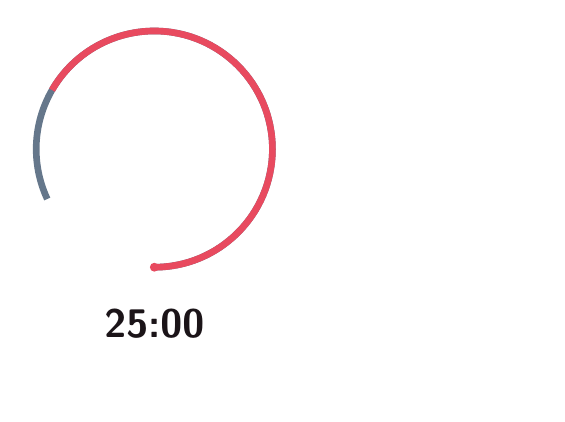
\begin{tikzpicture}
  % clock arc motif
  \begin{scope}
    \draw[line width=2.4pt, pastel!60!black] (0,0) arc[start angle=-90,end angle=205,radius=1.5];
    \draw[line width=2.4pt, accent] (0,0) arc[start angle=-90,end angle=150,radius=1.5];
    \fill[accent] (0,0) circle (1.6pt);
    \node[font=\sffamily\bfseries\fontsize{15}{18}\selectfont, text=ink] at (0,-0.72) {25:00};
  \end{scope}
  \hspace{9mm}
  \begin{scope}[shift={(4.6,0)}]
    \foreach \i in {0,1,2,3}{
      \pgfmathsetmacro{\yy}{-0.55+\i*0.36}
      \fill[pastel!45!black] (0,\yy) circle (1.7pt);
    }
    \fill[accent] (0,-0.55) circle (2.3pt);
    \fill[accent] (0,-0.19) circle (2.3pt);
    \fill[accent] (0,0.17) circle (2.3pt);
    \fill[accent] (0,0.53) circle (2.3pt);
    \node[font=\sffamily\bfseries\fontsize{15}{18}\selectfont, text=ink] at (0,-1.32) {4};
  \end{scope}
\end{tikzpicture}

\vspace{10mm}
\end{center}

\begin{center}
\begin{minipage}{0.86\linewidth}
\centering\small\sffamily\color{softink}
Fourteen files. Two complete user interfaces. One timer state machine that knows
nothing about windows, menus, or graphics.

\medskip

This document explains how the code fits together, using diagrams instead of prose
wherever a diagram can carry the idea. Every file, field, and control-flow path
described here is taken from the source tree in \file{src/}.
\end{minipage}
\end{center}

\vspace{6mm}

\begin{center}
\begin{minipage}{0.92\linewidth}
\small
\begin{center}
\begin{tabular}{@{}>{\bfseries\sffamily}p{34mm} p{96mm}@{}}
\toprule
Read this part & You will understand \\
\midrule
\rowcolor{corefill!55}
1--3 & The three-layer split, the module map, and which code compiles on which platform \\
\rowcolor{corefill!55}
4--6 & The timer state machine, the Pomodoro cycle, and the monotonic clock \\
\rowcolor{corefill!55}
7--8 & The intent-flag pattern that lets the core stay platform-free \\
\rowcolor{corefill!55}
9--10 & Settings and statistics storage, including the fixed-size cache \\
\rowcolor{corefill!55}
11--13 & The AppKit shell, the egui shell, and how input reaches the timer \\
\rowcolor{corefill!55}
14--16 & Themes, the release build, and what the test suite actually proves \\
\bottomrule
\end{tabular}
\end{center}
\end{minipage}
\end{center}

\vfill
\begin{center}
\sffamily\footnotesize\color{softink}
\texttt{src/app.rs} \textbullet{} \texttt{src/timer.rs} \textbullet{} \texttt{src/config.rs}
\textbullet{} \texttt{src/stats.rs} \textbullet{} \texttt{src/mac\_shell.rs}
\textbullet{} \texttt{src/egui\_shell.rs} \textbullet{} \dots
\end{center}
\clearpage
\tableofcontents
\clearpage
\section{The one idea that explains everything}

Rusty Pomodoro is a Pomodoro timer. That part is easy. The interesting part is that it has
\emph{two entirely different user interfaces} --- a hand-built AppKit one and an egui
one --- and the timer logic is shared byte-for-byte between them.

That only works because of a strict layering rule, which is stated in the first line of
\file{src/mac\_shell.rs}:

\begin{lstlisting}[caption={The module's own doc comment states the contract.}]
//! Renderer-free macOS UI. Rust owns timer/storage; AppKit owns controls and drawing.
\end{lstlisting}

\subsection{The three layers}

\begin{figure}[H]
\centering
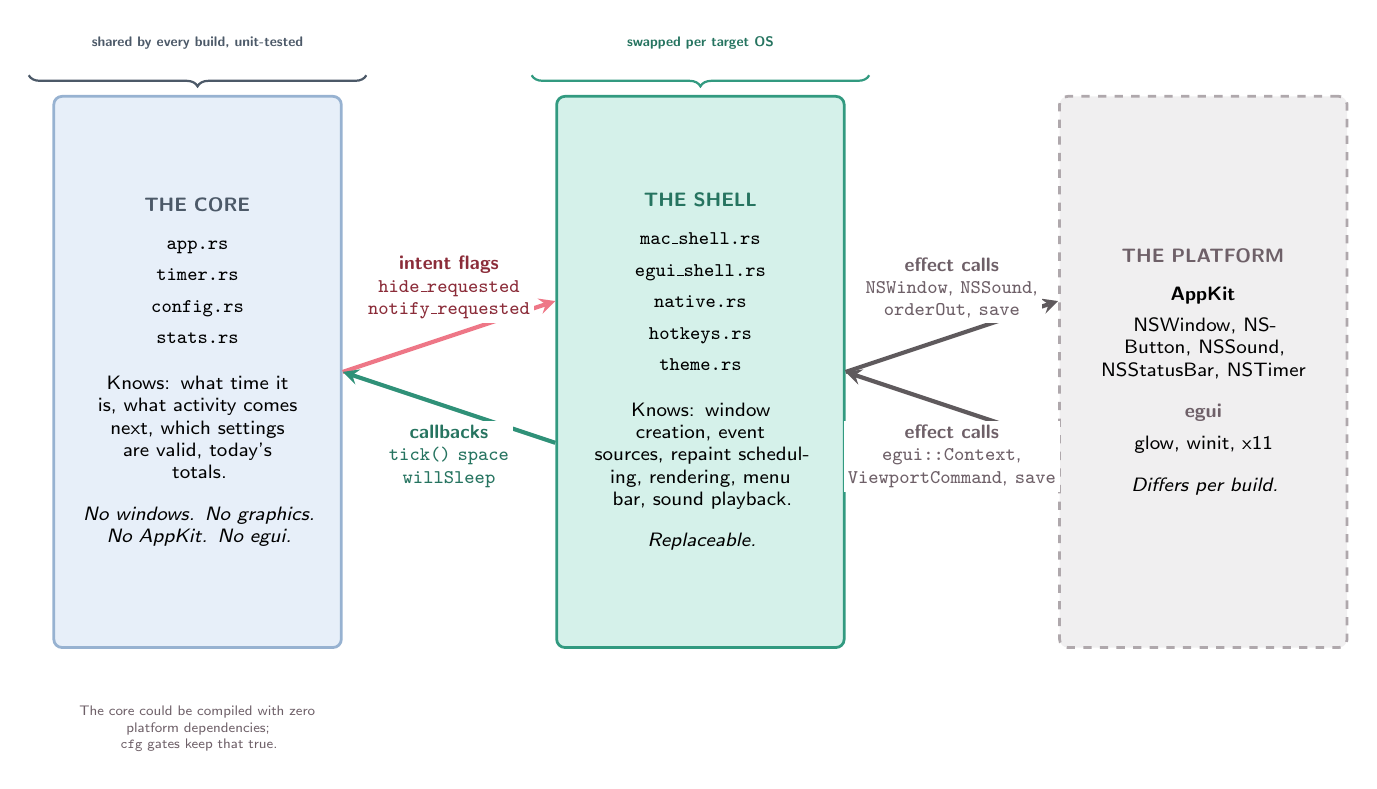
\begin{tikzpicture}[
  column/.style={rounded corners=3pt, line width=1pt, inner sep=5pt, align=center,
                 text width=33mm, minimum height=70mm, font=\scriptsize\sffamily},
]
  % ------------------------------------------------------------------ core
  \node[column, fill=corefill, draw=pastel!90!black] (core) at (0,0) {%
    \hd{\color{pastel!45!black}THE CORE}\\[2mm]
    \texttt{app.rs}\\[1.2mm] \texttt{timer.rs}\\[1.2mm]
    \texttt{config.rs}\\[1.2mm] \texttt{stats.rs}\\[3mm]
    Knows: what time it is, what activity comes\\next, which settings are valid,
    today's\\totals.\\[2.5mm]
    {\itshape No windows. No graphics.\\No AppKit. No egui.}};

  % ------------------------------------------------------------------ shell
  \node[column, fill=shellfill, draw=mint!80!black, right=27mm of core] (shell) {%
    \hd{\color{mint!60!black}THE SHELL}\\[2mm]
    \texttt{mac\_shell.rs}\\[1.2mm] \texttt{egui\_shell.rs}\\[1.2mm]
    \texttt{native.rs}\\[1.2mm] \texttt{hotkeys.rs}\\[1.2mm] \texttt{theme.rs}\\[3mm]
    Knows: window creation, event\\sources, repaint scheduling, rendering,
    menu\\bar, sound playback.\\[2.5mm]
    {\itshape Replaceable.}};

  % ------------------------------------------------------------------ os
  \node[column, fill=soft, draw=softink!55, dashed, right=27mm of shell] (os) {%
    \hd{\color{softink}THE PLATFORM}\\[2mm]
    \textbf{AppKit}\\[1.2mm]
    NSWindow, NSButton, NSSound,\\NSStatusBar, NSTimer\\[2.5mm]
    \hd{\color{softink}egui}\\[1.2mm]
    glow, winit, x11\\[2.5mm]
    {\itshape Differs per build.}};

  % ------------------------------------------------- core -> shell (intent)
  \draw[er, line width=1.5pt]
    (core.east) -- node[vlabel, midway, above=1.5mm, align=center, text=accent!60!black]
      {\textbf{intent flags}\\\texttt{hide\_requested}\\\texttt{notify\_requested}}
    ($(shell.west)+(0,9mm)$);

  % ------------------------------------------------- shell -> core (events)
  \draw[es, line width=1.5pt]
    ($(shell.west)+(0,-9mm)$) -- node[vlabel, midway, below=1.5mm, align=center, text=mint!60!black]
      {\textbf{callbacks}\\\texttt{tick()} \texttt{space}\\\texttt{willSleep}}
    (core.east);

  % ------------------------------------------------- shell -> platform
  \draw[e, line width=1.5pt]
    (shell.east) -- node[vlabel, midway, above=1.5mm, align=center]
      {\textbf{effect calls}\\\texttt{NSWindow}, \texttt{NSSound},\\\texttt{orderOut}, \texttt{save}}
    ($(os.west)+(0,9mm)$);
  \draw[e, line width=1.5pt]
    ($(os.west)+(0,-9mm)$) -- node[vlabel, midway, below=1.5mm, align=center]
      {\textbf{effect calls}\\\texttt{egui::Context},\\\texttt{ViewportCommand}, \texttt{save}}
    (shell.east);

  % ------------------------------------------------- group brackets
  \draw[decorate, decoration={brace, amplitude=4pt, mirror}, thick, pastel!45!black]
    ($(core.north west)+(-3mm,2.5mm)$) -- ($(core.north east)+(3mm,2.5mm)$)
    node[midway, above=2mm, font=\tiny\sffamily\bfseries, text=pastel!45!black]
      {shared by every build, unit-tested};

  \draw[decorate, decoration={brace, amplitude=4pt, mirror}, thick, mint!80!black]
    ($(shell.north west)+(-3mm,2.5mm)$) -- ($(shell.north east)+(3mm,2.5mm)$)
    node[midway, above=2mm, font=\tiny\sffamily\bfseries, text=mint!60!black]
      {swapped per target OS};

  \node[note, below=6mm of core.south, text width=33mm, font=\tiny\sffamily]
    {The core could be compiled with zero\\platform dependencies; \texttt{cfg}
     gates keep that true.};
\end{tikzpicture}
\caption{The layering. The core never calls a platform API; it only raises flags. The
shell reads them, performs the effect, and clears them with \texttt{std::mem::take}.}
\label{fig:layers}
\end{figure}

\subsection{The mechanism: five boolean fields}

The whole boundary is five public booleans on \file{App}, from \file{src/app.rs} lines 22--29:

\begin{lstlisting}[caption={Every side effect the core wants is a public boolean field.}]
pub hide_requested:   bool,   // shell should order the window out
pub show_requested:   bool,   // shell should bring the window forward
pub notify_requested: bool,   // shell should play the completion sound
pub tick_requested:   bool,   // shell should play the per-second tick sound
pub exit_requested:   bool,   // shell should terminate the process
\end{lstlisting}

The core never calls \texttt{NSBeep()} or \texttt{request\_repaint}. It only ever writes
\texttt{true}. The shell then calls \texttt{std::mem::take(\&mut app.notify\_requested)},
which reads the flag \emph{and} resets it to \texttt{false} in one step:

\begin{lstlisting}[caption={Both shells drain the flags identically, at the end of a frame.}]
// src/mac_shell.rs, refresh()
if std::mem::take(&mut app.hide_requested)   { views.window.orderOut(None); }
let show = std::mem::take(&mut app.show_requested);
if std::mem::take(&mut app.notify_requested) { play(app.settings.notification_sound); }
if std::mem::take(&mut app.tick_requested)   { play(Sound::Tink); }
\end{lstlisting}

Because the flag is cleared by the same read that tests it, an intent can never fire
twice. And because the core only writes booleans, it never needs to know whether a
shell exists at all --- the same \file{App} compiles inside both shells unmodified.

\begin{figure}[H]
\centering
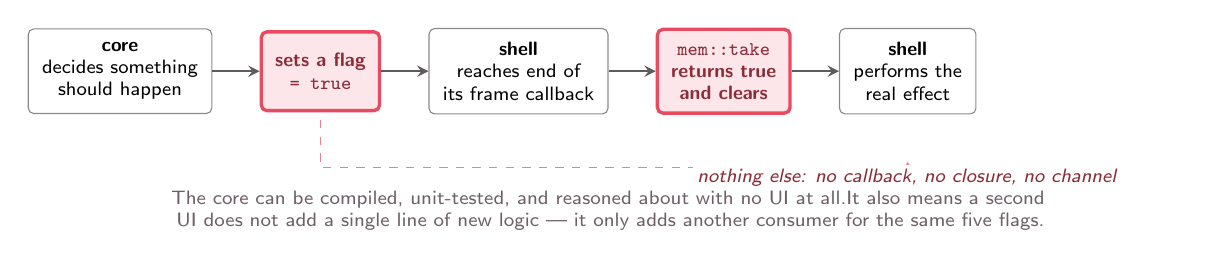
\begin{tikzpicture}[
  fw/.style={rounded corners=2pt,draw=ink!50,fill=white,align=center,
             inner sep=5pt,font=\scriptsize\sffamily,minimum height=10mm},
  key/.style={rounded corners=2pt,draw=accent,fill=accent!14,align=center,
              inner sep=5pt,line width=1.2pt,font=\scriptsize\sffamily\bfseries,
              text=accent!60!black,minimum height=10mm},
]
  \node[fw] (n1) {\textbf{core}\\ decides something\\ should happen};
  \node[key, right=6mm of n1] (n2) {sets a flag\\\texttt{= true}};
  \node[fw, right=6mm of n2] (n3) {\textbf{shell}\\ reaches end of\\its frame callback};
  \node[key, right=6mm of n3] (n4) {\texttt{mem::take}\\ returns true\\and clears};
  \node[fw, right=6mm of n4] (n5) {\textbf{shell}\\ performs the\\real effect};
  \foreach \a/\b in {n1/n2,n2/n3,n3/n4,n4/n5} \draw[e] (\a) -- (\b);

  \draw[ethin, dashed, accent!70] (n2.south) ++(0,-1mm) -- ++(0,-6mm)
        -| node[vlabel, below, pos=0.78, text=accent!60!black]
        {\emph{nothing else: no callback, no closure, no channel}}
        ($(n5.south)+(0,-6mm)$);

  \node[note, below=15mm of n3.5, text width=145mm] {%
    The core can be compiled, unit-tested, and reasoned about with no UI at all.%
    It also means a second UI does not add a single line of new logic --- it
    only adds another consumer for the same five flags.};
\end{tikzpicture}
\caption{The intent-flag protocol, as a five-step cycle.}
\label{fig:flags}
\end{figure}

\subsection{What one second of running looks like}

\begin{figure}[H]
\centering
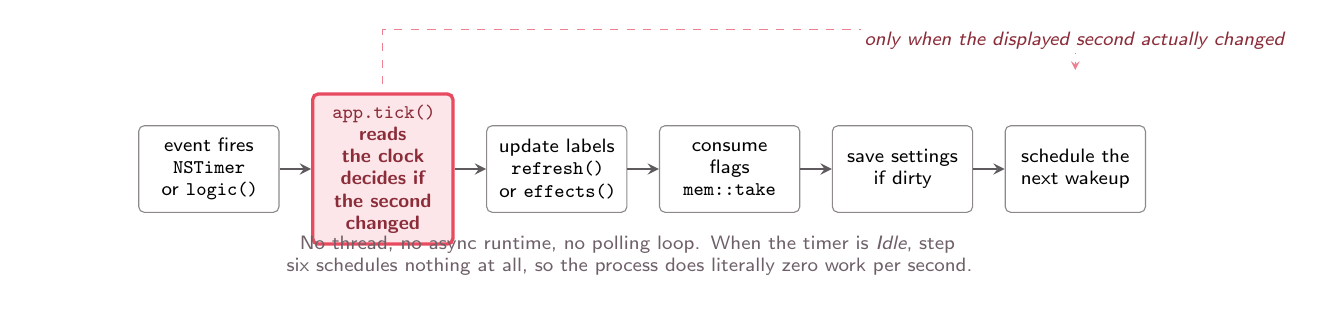
\begin{tikzpicture}[
  fw/.style={rounded corners=2pt,draw=ink!50,fill=white,align=center,
             inner sep=4pt,font=\scriptsize\sffamily,minimum height=11mm,text width=15mm},
  key/.style={fw, draw=accent, fill=accent!14, line width=1.2pt,
              text=accent!60!black, font=\scriptsize\sffamily\bfseries},
]
  \node[fw] (n1) {event fires\\\texttt{NSTimer}\\\scriptsize or \texttt{logic()}};
  \node[key, right=4mm of n1] (n2) {\texttt{app.tick()}\\\scriptsize reads the clock\\decides if the second\\changed};
  \node[fw, right=4mm of n2] (n3) {update labels\\\scriptsize \texttt{refresh()}\\\scriptsize or \texttt{effects()}};
  \node[fw, right=4mm of n3] (n4) {consume flags\\\scriptsize \texttt{mem::take}};
  \node[fw, right=4mm of n4] (n5) {save settings\\\scriptsize if dirty};
  \node[fw, right=4mm of n5] (n6) {schedule the\\\scriptsize next wakeup};
  \foreach \a/\b in {n1/n2,n2/n3,n3/n4,n4/n5,n5/n6} \draw[e] (\a) -- (\b);

  \draw[ethin, dashed, accent!70] (n2.north) ++(0,1mm) -- ++(0,7mm)
        -| node[vlabel, above, pos=0.80, text=accent!60!black]
        {\emph{only when the displayed second actually changed}}
        ($(n6.north)+(0,7mm)$);

  \node[note, below=8mm of n3.5, text width=150mm] {%
    No thread, no async runtime, no polling loop. When the timer is \emph{Idle},
    step six schedules nothing at all, so the process does literally zero work per second.};
\end{tikzpicture}
\caption{The per-second cycle in the AppKit shell. \texttt{refresh()} ends by arming
exactly one one-shot \texttt{NSTimer} for the instant the next displayed digit changes.}
\label{fig:second}
\end{figure}
\clearpage
\section{The module map}

\subsection{The core: four modules and two files on disk}

Every arrow below is a real \texttt{use crate::\ldots} in the source. Notice the
direction of dependency: \file{timer.rs} and \file{config.rs} do not know that
\file{App} exists. \file{App} is the only thing that knows about all of them.

\begin{figure}[H]
\centering
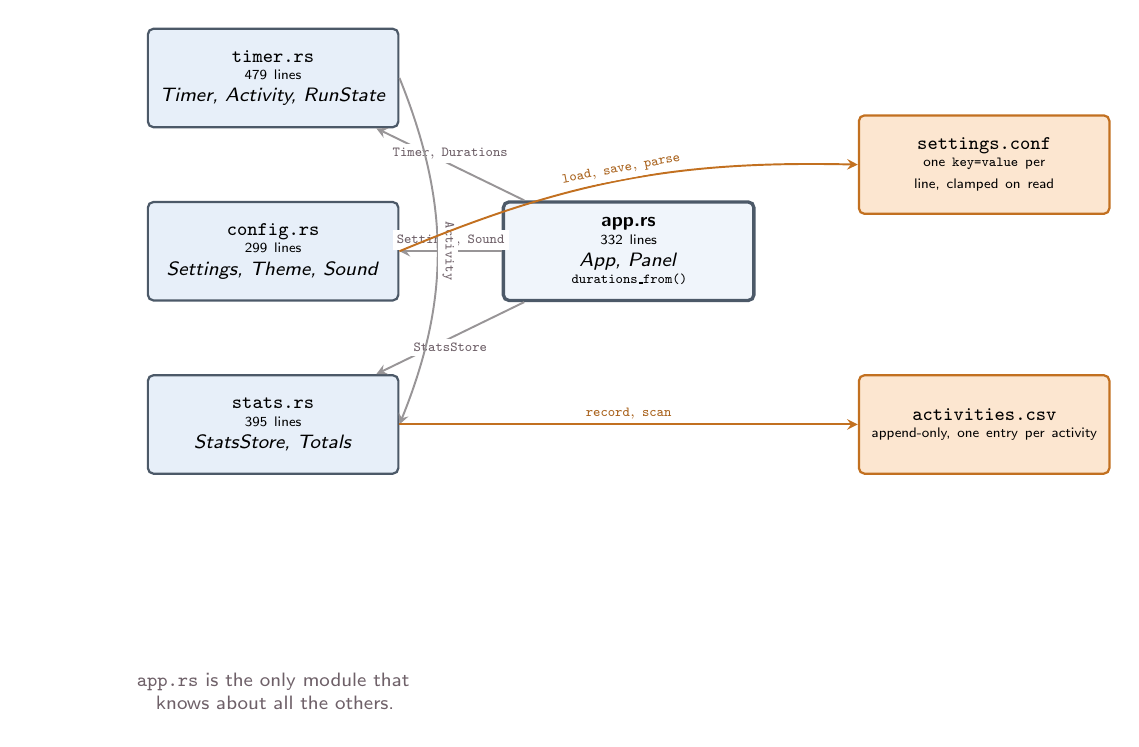
\begin{tikzpicture}[x=1.05cm,y=1cm,
  core/.style={rounded corners=2pt, draw=pastel!45!black, fill=corefill, align=center,
               inner sep=4pt, line width=0.8pt, font=\scriptsize\sffamily,
               minimum height=1.25cm, text width=2.9cm},
  data/.style={rounded corners=2pt, draw=mandarin!70!black, fill=datafill, align=center,
               inner sep=4pt, line width=0.8pt, font=\scriptsize\sffamily,
               minimum height=1.25cm, text width=2.9cm, draw=mandarin!80!black},
  e/.style={-stealth, draw=ink!45, line width=0.7pt},
  ed/.style={-stealth, draw=mandarin!80!black, line width=0.7pt},
]
  \node[core] (timer)  at (0,3.1) {\texttt{timer.rs}\\[-0.6mm]{\tiny 479 lines}\\\textit{Timer, Activity, RunState}};
  \node[core] (config) at (0,0.9) {\texttt{config.rs}\\[-0.6mm]{\tiny 299 lines}\\\textit{Settings, Theme, Sound}};
  \node[core] (stats)  at (0,-1.3) {\texttt{stats.rs}\\[-0.6mm]{\tiny 395 lines}\\\textit{StatsStore, Totals}};
  \node[core, fill=corefill!60!white, line width=1.2pt] (app)
        at (4.3,0.9) {\textbf{app.rs}\\[-0.6mm]{\tiny 332 lines}\\\textit{App, Panel}\\[-0.6mm]{\tiny \texttt{durations\_from()}}};

  \node[data] (conf) at (8.6,2.0) {\texttt{settings.conf}\\[-0.6mm]{\tiny one \texttt{key=value} per line, clamped on read}};
  \node[data] (csv)  at (8.6,-1.3) {\texttt{activities.csv}\\[-0.6mm]{\tiny append-only, one entry per activity}};

  \draw[e] (app) -- node[vlabel, above, font=\tiny] {\texttt{Timer}, \texttt{Durations}} (timer);
  \draw[e] (app) -- node[vlabel, above, font=\tiny] {\texttt{Settings}, \texttt{Sound}} (config);
  \draw[e] (app) -- node[vlabel, below, font=\tiny] {\texttt{StatsStore}} (stats);
  \draw[e] (timer.east) to[bend left=22] node[vlabel, above, font=\tiny, sloped] {\texttt{Activity}} (stats.east);
  \draw[ed] (config.east) to[bend left=12] node[vlabel, above, font=\tiny, sloped, text=mandarin!70!black] {\texttt{load}, \texttt{save}, \texttt{parse}} (conf.west);
  \draw[ed] (stats.east) -- node[vlabel, above, font=\tiny, text=mandarin!70!black] {\texttt{record}, \texttt{scan}} (csv.west);

  \node[note, below=2.4cm of stats, text width=6.0cm] {%
    \texttt{app.rs} is the only module that knows about all the others.};
\end{tikzpicture}
\caption{The platform-free core. \file{timer.rs} imports only \texttt{std::time}
and, on macOS, two Mach functions declared by hand. \file{config.rs} and
\file{stats.rs} touch only \texttt{std::fs} and \texttt{libc}.}
\label{fig:core-map}
\end{figure}

\subsection{The shells: two of them, plus their helpers}

\begin{figure}[H]
\centering
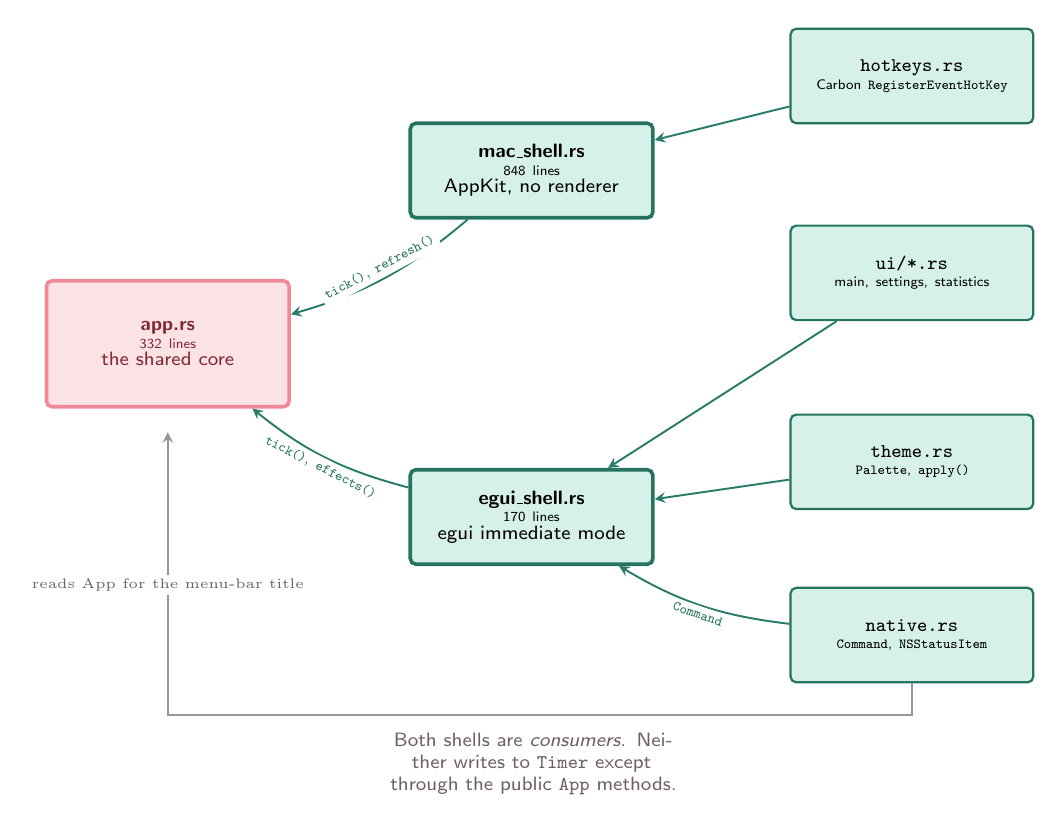
\begin{tikzpicture}[x=1.05cm,y=1cm,
  shell/.style={rounded corners=2pt, draw=mint!60!black, fill=shellfill, align=center,
               inner sep=4pt, line width=0.8pt, font=\scriptsize\sffamily,
               minimum height=1.2cm, text width=2.8cm},
  nat/.style={rounded corners=2pt, draw=accent!65, fill=intentfill, align=center,
              inner sep=4pt, line width=0.8pt, font=\scriptsize\sffamily,
              minimum height=1.2cm, text width=2.8cm, text=accent!55!black},
  es/.style={-stealth, draw=mint!65!black, line width=0.7pt},
  e/.style={-stealth, draw=ink!45, line width=0.7pt},
]
  % targets
  \node[nat, minimum height=1.6cm, line width=1.3pt] (app)
        at (0,0) {\textbf{app.rs}\\[-0.6mm]{\tiny 332 lines}\\[-0.6mm]the shared core};

  % the two shells
  \node[shell, line width=1.3pt] (mac)  at (4.4,2.2)
        {\textbf{mac\_shell.rs}\\[-0.6mm]{\tiny 848 lines}\\[-0.6mm]AppKit, no renderer};
  \node[shell, line width=1.3pt] (egui) at (4.4,-2.2)
        {\textbf{egui\_shell.rs}\\[-0.6mm]{\tiny 170 lines}\\[-0.6mm]egui immediate mode};

  % helpers
  \node[shell] (hotkeys) at (9.0,3.4) {\texttt{hotkeys.rs}\\[-0.6mm]{\tiny Carbon \texttt{RegisterEventHotKey}}};
  \node[shell] (ui)     at (9.0,0.9) {\texttt{ui/*.rs}\\[-0.6mm]{\tiny main, settings, statistics}};
  \node[shell] (theme)  at (9.0,-1.5) {\texttt{theme.rs}\\[-0.6mm]{\tiny \texttt{Palette}, \texttt{apply()}}};
  \node[shell] (native) at (9.0,-3.7) {\texttt{native.rs}\\[-0.6mm]{\tiny \texttt{Command}, \texttt{NSStatusItem}}};

  \draw[es] (mac)  to[bend left=12] node[vlabel, above, font=\tiny, sloped, text=mint!60!black] {\texttt{tick()}, \texttt{refresh()}} (app);
  \draw[es] (egui) to[bend left=12] node[vlabel, below, font=\tiny, sloped, text=mint!60!black] {\texttt{tick()}, \texttt{effects()}} (app);
  \draw[es] (hotkeys) -- (mac);
  \draw[es] (ui)     -- (egui);
  \draw[es] (theme)  -- (egui);
  \draw[es] (native) to[bend left=12] node[vlabel, below, font=\tiny, sloped, text=mint!60!black] {\texttt{Command}} (egui);
  \draw[e]  (native.south) -- ++(0,-4mm) -| node[vlabel, below, font=\tiny, pos=0.75]
        {reads App for the menu-bar title} ($(app.south)+(0,-3mm)$);

  \node[note, below=2.0cm of egui, text width=4.4cm] {%
    Both shells are \emph{consumers}. Neither writes to \texttt{Timer} except
    through the public \texttt{App} methods.};
\end{tikzpicture}
\caption{Shell cluster. \file{native.rs} is a thin AppKit bridge that turns menu
clicks and power notifications into an enum value, then queues it for the next frame.}
\label{fig:shell-map}
\end{figure}

\subsection{Line counts}

\begin{figure}[H]
\centering
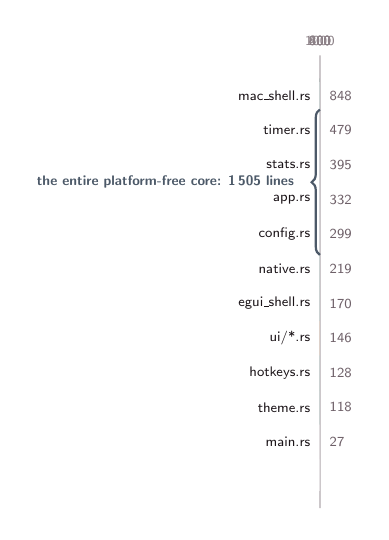
\begin{tikzpicture}[x=0.000000000000000000000001mm,y=4.4mm]
  % frame + gridlines
  \draw[draw=softink!35, line width=0.5pt, rounded corners=2pt] (0,0) rectangle (-5320,-13);
  \foreach \v in {200,400,600,800,1000}
    \draw[softink!18, line width=0.4pt] (\v,-12.4) -- (\v,-0.6);
  \foreach \lab/\v in {200/200,400/400,600/600,800/800,1000/1000}
    \node[anchor=south, font=\tiny\sffamily, text=softink!80] at (\v,0.15) {\lab};

  % bars, tallest first: y position = index, width = lines
  \newcommand{\drawbar}[3]{\fill[#2] (0,{#1-0.5}) rectangle (#3,{#1+0.5});}
  \newcommand{\rowlab}[2]{\node[anchor=east, font=\tiny\sffamily, text=ink] at (-20,#1) {#2};}
  \newcommand{\rowval}[2]{\node[anchor=west, font=\tiny\sffamily, text=softink] at (-4320,#1) {#2};}

  \rowlab{-1}{mac\_shell.rs}   \drawbar{-1}{mint!55!black}{848}      \rowval{-1}{848}
  \rowlab{-2}{timer.rs}        \drawbar{-2}{pastel!55!black}{479}    \rowval{-2}{479}
  \rowlab{-3}{stats.rs}        \drawbar{-3}{pastel!55!black}{395}    \rowval{-3}{395}
  \rowlab{-4}{app.rs}          \drawbar{-4}{pastel!55!black}{332}    \rowval{-4}{332}
  \rowlab{-5}{config.rs}       \drawbar{-5}{pastel!55!black}{299}    \rowval{-5}{299}
  \rowlab{-6}{native.rs}       \drawbar{-6}{mint!55!black}{219}      \rowval{-6}{219}
  \rowlab{-7}{egui\_shell.rs}  \drawbar{-7}{mint!55!black}{170}      \rowval{-7}{170}
  \rowlab{-8}{ui/*.rs}         \drawbar{-8}{mandarin!70!black}{146}  \rowval{-8}{146}
  \rowlab{-9}{hotkeys.rs}      \drawbar{-9}{mint!55!black}{128}      \rowval{-9}{128}
  \rowlab{-10}{theme.rs}       \drawbar{-10}{mint!55!black}{118}     \rowval{-10}{118}
  \rowlab{-11}{main.rs}        \drawbar{-11}{softink!45}{27}         \rowval{-11}{27}

  % bracket marking the core
  \draw[decorate, decoration={brace, amplitude=3pt}, thick, pastel!45!black]
    (-12,-5.6) -- (-12,-1.4) node[midway, left=2mm, font=\tiny\sffamily\bfseries, text=pastel!45!black]
    {the entire platform-free core: 1\,505 lines};
\end{tikzpicture}
\caption{Source size by file. The five pastel bars are the core; they compile and test
without a window, an image, or a sound card.}
\label{fig:loc}
\end{figure}

\subsection{Two shells, side by side}

\begin{table}[H]
\centering\small
\begin{tabular}{@{}p{32mm} p{54mm} p{56mm}@{}}
\toprule
& \textbf{mac\_shell.rs} (default on macOS) & \textbf{egui\_shell.rs} (\texttt{--features egui-ui}) \\
\midrule
Rendering & none --- the OS draws the controls & egui immediate mode, \texttt{glow} backend \\
Event source & one one-shot \texttt{NSTimer} & egui repaint requests \\
Frame callback & \texttt{refresh()} & \texttt{effects()}, called from \texttt{logic()} and \texttt{ui()} \\
Menu bar & real \texttt{NSStatusBar} item & \texttt{native.rs} \texttt{NSStatusItem} \\
Global keys & Carbon \texttt{RegisterEventHotKey} & none (app-focused keys only) \\
Sound & \texttt{NSSound::soundNamed} & \texttt{native::play} on macOS, silent elsewhere \\
Window & fixed 380$\times$300, no resize & 360$\times$440 minimum, 400$\times$460 default \\
Themes & one coloured label per theme & five full \texttt{Palette}s via \file{theme.rs} \\
Panels & real \texttt{NSWindow}s, built lazily & \texttt{egui::Window}s \\
\bottomrule
\end{tabular}
\caption{Both shells drive the identical \file{App}. The differences are entirely about
how pixels and events arrive, never about what the timer does.}
\end{table}
\clearpage
\section{One binary, two personalities: the \texttt{cfg} switch}

\file{src/main.rs} is 27 lines and does nothing but decide which shell to compile.
Reading it top to bottom explains the whole build matrix.

\begin{lstlisting}[caption={\file{src/main.rs}, complete.}]
#[cfg(feature = "egui-ui")] fn main() -> eframe::Result { egui_shell::run() }

#[cfg(all(target_os = "macos", not(feature = "egui-ui")))]
fn main() { mac_shell::run(); }

#[cfg(all(not(target_os = "macos"), not(feature = "egui-ui")))]
compile_error!("Build on Windows/Linux with --features egui-ui.");
\end{lstlisting}

\subsection{The matrix this produces}

\begin{figure}[H]
\centering
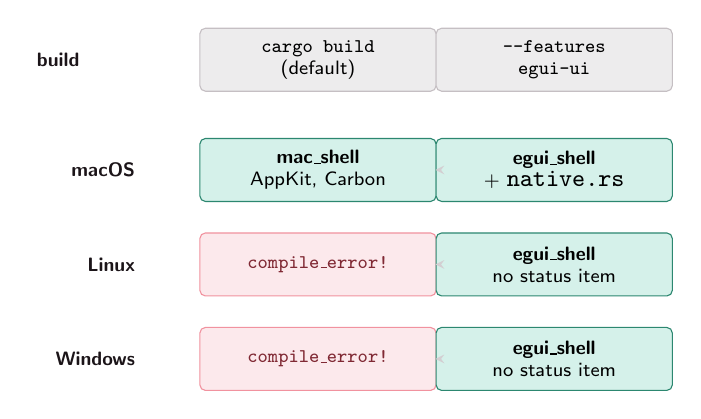
\begin{tikzpicture}[
  head/.style={font=\scriptsize\sffamily\bfseries, text=ink},
  cellok/.style={rounded corners=2pt, draw=mint!70!black, fill=mint!22, minimum height=8mm,
                 minimum width=30mm, align=center, font=\scriptsize\sffamily},
  cellno/.style={rounded corners=2pt, draw=accent!60, fill=accent!12, minimum height=8mm,
                 minimum width=30mm, align=center, font=\scriptsize\sffamily, text=accent!55!black},
]
  \node[head] at (-1.7,2.6) {build};
  \node[cellok, fill=ink!8, draw=softink!40] (h1) at (1.6,2.6) {\texttt{cargo build}\\\scriptsize (default)};
  \node[cellok, fill=ink!8, draw=softink!40] (h2) at (4.6,2.6) {\texttt{--features}\\\scriptsize \texttt{egui-ui}};

  % --- row 1: macOS default
  \node[head, anchor=east] at (-0.6,1.2) {macOS};
  \node[cellok] (r1a) at (1.6,1.2) {\textbf{mac\_shell}\\\scriptsize AppKit, Carbon};
  \node[cellok] (r1b) at (4.6,1.2) {\textbf{egui\_shell}\\\scriptsize + \file{native.rs}};

  % --- row 2: linux default
  \node[head, anchor=east] at (-0.6,0.0) {Linux};
  \node[cellno] (r2a) at (1.6,0.0) {\texttt{compile\_error!}};
  \node[cellok] (r2b) at (4.6,0.0) {\textbf{egui\_shell}\\\scriptsize no status item};

  % --- row 3: windows default
  \node[head, anchor=east] at (-0.6,-1.2) {Windows};
  \node[cellno] (r3a) at (1.6,-1.2) {\texttt{compile\_error!}};
  \node[cellok] (r3b) at (4.6,-1.2) {\textbf{egui\_shell}\\\scriptsize no status item};

  \foreach \a/\b in {r1a/r1b,r2a/r2b,r3a/r3b} \draw[ethin, softink!30] (\a) -- (\b);

  \end{tikzpicture}

\vspace{2mm}
{\small
\textcolor{pastel!45!black}{\texttt{app}, \texttt{timer}, \texttt{config}, \texttt{stats}}
\quad\textcolor{softink}{|}\quad
\textcolor{mint!60!black}{\texttt{mac\_shell}, \texttt{hotkeys}} (macOS, no feature)\\[1mm]
\textcolor{accent!55!black}{\texttt{egui\_shell}, \texttt{native}, \texttt{theme}, \texttt{ui::*}} (with feature)
}
\caption{The three build outcomes. The four core modules are compiled in every row;
only the shell differs.}
\label{fig:cfg}
\end{figure}

\subsection{What each module is gated on}

\begin{table}[H]
\centering\small
\begin{tabular}{@{}p{34mm} p{40mm} p{66mm}@{}}
\toprule
\textbf{Gate on \texttt{mod}} & \textbf{Compiled when} & \textbf{Reason it exists} \\
\midrule
\texttt{app}, \texttt{config}, \texttt{stats}, \texttt{timer} & always & the portable core \\
\texttt{mac\_shell}, \texttt{hotkeys} & \texttt{macOS} \texttt{\&\& !egui-ui} & the default macOS build \\
\texttt{egui\_shell}, \texttt{native}, \texttt{theme}, \texttt{ui} & \texttt{feature = "egui-ui"} & the cross-platform build \\
\bottomrule
\end{tabular}
\caption{The full \texttt{mod} list from \file{main.rs}. Nothing is gated on a runtime
condition: the choice is made once, at compile time.}
\end{table}

\subsection{Why a Cargo feature rather than a runtime check}

\begin{figure}[H]
\centering
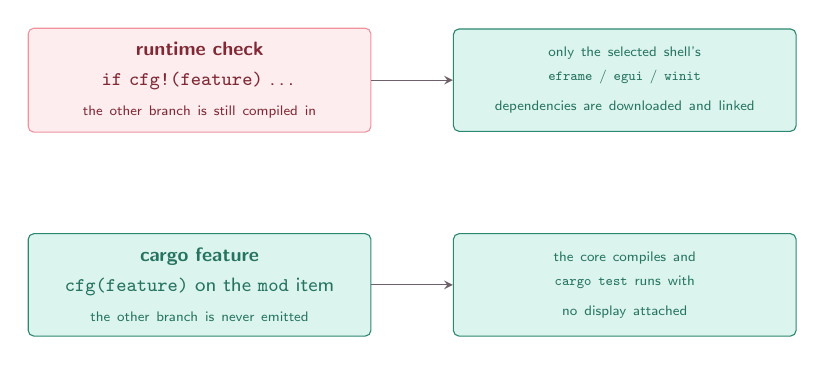
\begin{tikzpicture}[
  box/.style={rounded corners=2pt,draw=ink!45,fill=white,align=center,inner sep=5pt,
              font=\scriptsize\sffamily,text width=40mm,minimum height=13mm},
  good/.style={box,draw=mint!70!black,fill=mint!18,text=mint!60!black},
  bad/.style={box,draw=accent!60,fill=accent!10,text=accent!55!black},
]
  \node[bad]  (a) at (0,0) {\textbf{runtime check}\\[1mm]\texttt{if cfg!(feature)} \dots\\[1mm]
     {\tiny the other branch is still compiled in}};
  \node[good] (b) at (0,-2.6) {\textbf{cargo feature}\\[1mm]\texttt{cfg(feature)} on the \texttt{mod} item\\[1mm]
     {\tiny the other branch is never emitted}};

  \node[good] (c) at (5.4,0) {\tiny only the selected shell's\\[1mm]\code{eframe} / \code{egui} / \code{winit}\\[1mm]
     dependencies are downloaded and linked};
  \node[good] (d) at (5.4,-2.6) {\tiny the core compiles and\\[1mm]\code{cargo test} runs with\\[1mm]no display attached};

  \draw[ethin, softink] (a.east) -- (c.west);
  \draw[ethin, softink] (b.east) -- (d.west);
\end{tikzpicture}
\caption{A Cargo feature removes the other branch at compile time, so the default macOS
build never links \texttt{eframe}, \texttt{egui}, or \texttt{winit} at all.}
\label{fig:whyfeature}
\end{figure}

\begin{lstlisting}[caption={\file{Cargo.toml}. The whole egui stack is optional, and
\code{default = []} means an ordinary \code{cargo build} produces the AppKit app.}]
[features]
default = []
egui-ui = ["dep:eframe", "dep:egui"]

[dependencies]
eframe = { version = "0.36", optional = true, default-features = false, features = ["glow", "x11"] }
egui   = { version = "0.36.2", optional = true, default-features = false }
\end{lstlisting}

\keybox{mint}{%
\textbf{Three deliberate cuts in \code{default-features = false}.}
\code{eframe} would normally pull in an accessibility stack, a link handler, a web
screen reader, and a serde-backed persistence layer; \code{egui} would pull in a
default font atlas with emoji fallbacks. All of it is disabled. The one 302\,KiB
\file{Hack-Regular.ttf} in \file{assets/} is embedded with \texttt{include\_bytes!}
and installed as the \emph{only} font for both the proportional and monospace
families.}
\clearpage
\section{The timer state machine}

\file{src/timer.rs} is 479 lines and imports exactly one thing:
\texttt{std::time::Duration}. It is the only file in the project that decides what
happens next, and it has no idea a user interface exists.

\subsection{Two orthogonal dimensions}

The machine has two independent state variables, and almost every bug in a hand-rolled
timer comes from confusing them.

\begin{figure}[H]
\centering
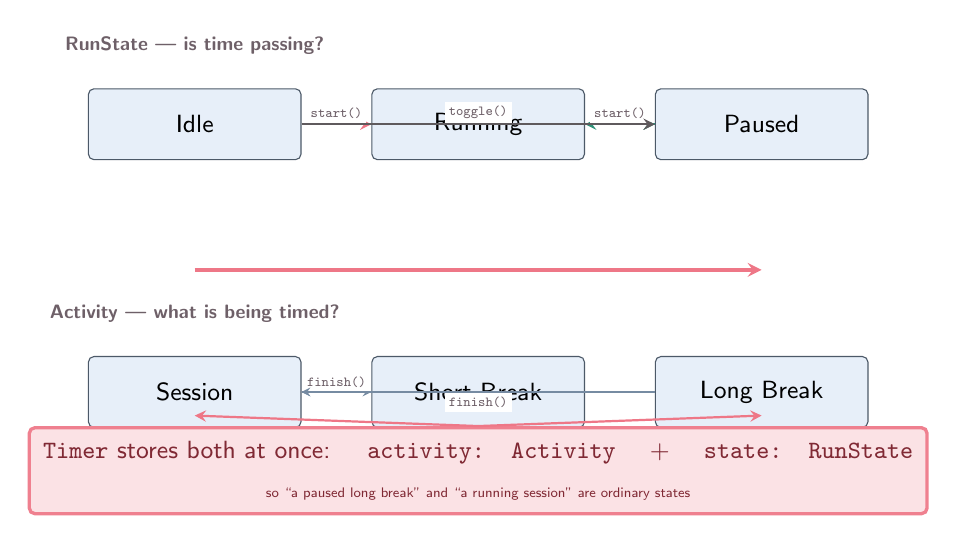
\begin{tikzpicture}[
  st/.style={rounded corners=2pt,draw=pastel!45!black,fill=corefill,align=center,
             inner sep=5pt,font=\small\sffamily,minimum height=9mm,minimum width=27mm},
  stc/.style={st,draw=accent!70,fill=accent!16,text=accent!55!black,line width=1.2pt},
  hd/.style={font=\scriptsize\sffamily\bfseries,text=softink},
  cell/.style={font=\tiny\sffamily,align=center,inner sep=3pt},
]
  % RunState row
  \node[hd] at (-3.6,2.5) {\textbf{RunState} --- is time passing?};
  \node[st] (idle)   at (-3.6,1.5) {Idle};
  \node[st] (run)    at ( 0.0,1.5) {Running};
  \node[st] (paused) at ( 3.6,1.5) {Paused};

  % Activity row
  \node[hd] at (-3.6,-0.9) {\textbf{Activity} --- what is being timed?};
  \node[st] (sess)  at (-3.6,-1.9) {Session};
  \node[st] (sb)    at ( 0.0,-1.9) {Short Break};
  \node[st] (lb)    at ( 3.6,-1.9) {Long Break};

  % arrows within RunState
  \draw[er] (idle)  -- node[vlabel, above, font=\tiny] {\texttt{start()}} (run);
  \draw[es] (run)   -- node[vlabel, above, font=\tiny] {\texttt{pause()}} (paused);
  \draw[es] (paused)-- node[vlabel, above, font=\tiny] {\texttt{start()}} (run);
  \draw[e]  (idle)  -- node[vlabel, above, font=\tiny] {\texttt{toggle()}} (paused);

  % arrows within Activity
  \draw[ethin, pastel!70!black] (sess) -- node[vlabel, above, font=\tiny] {\texttt{finish()}} (sb);
  \draw[ethin, pastel!70!black] (sb)   -- node[vlabel, above, font=\tiny] {\texttt{finish()}} (sess);
  \draw[ethin, pastel!70!black] (sess) to[bend right=28] node[vlabel, below, font=\tiny, text=accent!55!black]
        {\texttt{finish()} at a cycle boundary} (lb);
  \draw[ethin, pastel!70!black] (lb)   -- node[vlabel, below, font=\tiny] {\texttt{finish()}} (sess);

  % the cross product
  \draw[er, very thick] (-3.6,-0.35) -- (3.6,-0.35) node[midway, above, font=\tiny] {};
  \node[stc, minimum width=74mm] (prod) at (0,-2.9)
    {\texttt{Timer} stores both at once: \quad \texttt{activity: Activity} \quad + \quad \texttt{state: RunState}\\[1mm]
     \tiny so ``a paused long break'' and ``a running session'' are ordinary states};
  \draw[er] (prod.north) -- (-3.6,-2.2);
  \draw[er] (prod.north) -- (3.6,-2.2);
\end{tikzpicture}
\caption{Tomito-RS keeps a \emph{product} state, not a flat enum. ``Idle Session'' and
``Running Session'' share the same activity and the same duration but differ entirely
in behaviour, so splitting them keeps each rule in one place.}
\label{fig:states}
\end{figure}

\subsection{Time is not stored; it is derived}

This is the single most important design decision in \file{timer.rs}. The struct does
\emph{not} keep a countdown that is decremented once a second. It keeps a timestamp and
asks the clock:

\begin{lstlisting}[caption={The four lines that make \texttt{Timer} tick-free.}]
pub fn elapsed(&self) -> Duration {
    match self.started_at {
        Some(start) => self.elapsed + start.elapsed(),   // running: frozen + live
        None        => self.elapsed,                      // idle/paused: frozen only
    }
}
pub fn remaining(&self) -> Duration {
    self.duration.saturating_sub(self.elapsed())          // saturates: no underflow
}
\end{lstlisting}

\begin{figure}[H]
\centering
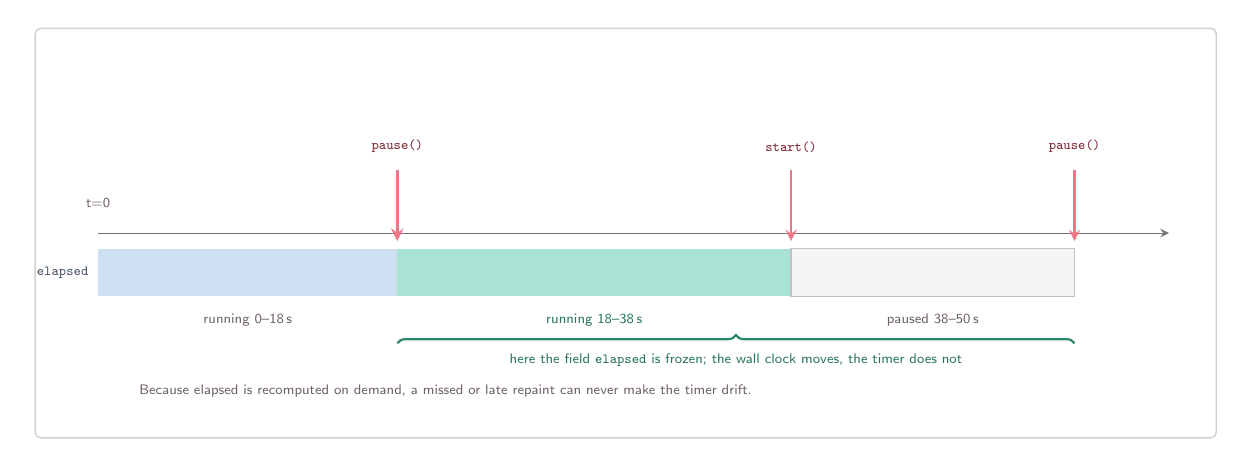
\begin{tikzpicture}[x=1mm,y=1mm]
  \draw[draw=softink!30,line width=0.5pt,rounded corners=2pt] (0,0) rectangle (150,52);
  % axis
  \draw[-stealth, draw=ink!60] (8,26) -- (144,26);
  \node[anchor=south,font=\tiny\sffamily,text=softink] at (8,28) {t=0};

  % frozen segment
  \fill[pastel!55] (8,18) rectangle (46,24);
  \node[anchor=east,font=\tiny\sffamily,text=pastel!45!black] at (8,21) {\texttt{elapsed}};
  \node[anchor=north,font=\tiny\sffamily,text=softink] at (27,17) {running 0--18\,s};

  % live segment
  \fill[mint!45] (46,18) rectangle (96,24);
  \node[anchor=north,font=\tiny\sffamily,text=mint!60!black] at (71,17) {running 18--38\,s};
  \draw[er, line width=1pt] (46,34) -- (46,25);
  \node[anchor=south,font=\tiny\sffamily,text=accent!55!black] at (46,35) {\texttt{pause()}};

  % paused segment
  \fill[soft!60, draw=softink!40] (96,18) rectangle (132,24);
  \node[anchor=north,font=\tiny\sffamily,text=softink] at (114,17) {paused 38--50\,s};
  \draw[er] (96,34) -- (96,25);
  \node[anchor=south,font=\tiny\sffamily,text=accent!55!black] at (96,35) {\texttt{start()}};
  \draw[er] (132,34) -- (132,25);
  \node[anchor=south,font=\tiny\sffamily,text=accent!55!black] at (132,35) {\texttt{pause()}};

  % annotation
  \draw[decorate,decoration={brace,amplitude=3pt}, thick, mint!70!black]
     (46,12) -- (132,12) node[midway,below,font=\tiny\sffamily,text=mint!60!black]
     {here the field \texttt{elapsed} is frozen; the wall clock moves, the timer does not};
  \node[anchor=west,font=\tiny\sffamily,text=softink,align=left] at (12,6)
    {Because elapsed is recomputed on demand, a missed or late repaint can never make the timer drift.};
\end{tikzpicture}
\caption{The two-part elapsed time. \texttt{elapsed} holds the accumulated total;
\texttt{started\_at} holds the moment the current running stretch began.}
\label{fig:elapsed}
\end{figure}

Three consequences follow for free:

\begin{itemize}[leftmargin=1.4em,itemsep=0.3em]
  \item \textbf{No drift.} There is no ``subtract one every tick'', so a late wake-up, a
        blocked main thread, or a machine that was busy cannot make the timer lose time.
  \item \textbf{Pause is exact.} \texttt{pause()} folds the live part into the frozen part
        and drops the timestamp; the number cannot move afterwards.
  \item \textbf{Overtime falls out.} \texttt{remaining()} uses \texttt{saturating\_sub}, so
        once elapsed passes duration it simply pins at zero and
        \texttt{elapsed() - duration()} becomes the overtime count.
\end{itemize}

\subsection{The transition table}

\begin{table}[H]
\centering\small
\small\small\small\small\small\small\small\small\small\small\small\small\small\small\small\small\small\small\small\small\small\small\small\small\small\small\small\small\small\small\small\small\small\small\small\small\small\small\small\small\small\small\small\small\small\small\small\small\small\small\small\small\small\small\small\small\small\small\small\small\small\small\small\small\small\small\small\small\small\small\small\small\small\small\small\small\small\small\small\small\small\small\small\small\small\small\small\small\small\small\small\small\small\small\small\small\small\small\small\small\small\small\small\small\small\small\small\small\small\small\small\small\small\small\small\small\small\small\small\small\small\small\small\small\small\small\small\begin{tabular}{@{}p{20mm} p{18mm} p{20mm} p{70mm}@{}}
\toprule
\textbf{Method} & \textbf{From} & \textbf{To} & \textbf{What it does to the fields} \\
\midrule
\texttt{start()} & Idle / Paused & Running & if Idle \emph{and} elapsed $\ge$ duration, reset elapsed to 0; set \texttt{started\_at = Clock::now()} \\
\texttt{pause()} & Running & Paused & \texttt{elapsed += started\_at.elapsed()}, then \texttt{started\_at = None} \\
\texttt{toggle()} & any & flip & dispatches to \texttt{pause()} or \texttt{start()} \\
\texttt{stop()} & any & Idle & \texttt{elapsed = 0}, \texttt{started\_at = None}. Activity is \emph{kept} \\
\texttt{restart()} & any & unchanged & \texttt{elapsed = 0}; re-stamp \texttt{started\_at} only if Running \\
\texttt{skip()} & any & Idle, next activity & \texttt{advance(Skipped)} \\
\texttt{finish()} & any & Idle, next activity & \texttt{advance(Finished)} \\
\texttt{apply\_settings()} & any & unchanged & folds running time in, then recomputes \texttt{duration} \\
\bottomrule
\end{tabular}
\caption{\file{timer.rs}. \texttt{stop} and \texttt{restart} are the pair people confuse:
stop rewinds \emph{and} goes Idle, restart rewinds but keeps Running.}
\end{table}

\subsection{\texttt{advance}: where the Pomodoro rules live}

\begin{lstlisting}[caption={\file{timer.rs} lines 270--299. This function is the Pomodoro
specification; nothing else in the codebase contains a rule.}]
fn advance(&mut self, completion: Completion) -> Completion {
    let finished = self.activity;
    if completion == Completion::Finished && finished == Activity::Session {
        self.completed_sessions = self.completed_sessions.saturating_add(1);
    }
    let next = match finished {
        Activity::Session => {
            let cycle = self.settings.long_break_cycle.max(1);
            let due_long = completion == Completion::Finished
                && self.completed_sessions > 0
                && self.completed_sessions.is_multiple_of(cycle);
            if self.settings.disable_breaks      { Activity::Session }
            else if due_long && !self.settings.disable_long_breaks { Activity::LongBreak }
            else                                 { Activity::ShortBreak }
        }
        Activity::ShortBreak | Activity::LongBreak => Activity::Session,
    };
    self.activity = next;
    self.duration = duration_for(next, self.settings);
    self.elapsed = Duration::ZERO;
    self.started_at = None;
    self.state = RunState::Idle;
    completion
}
\end{lstlisting}

\begin{figure}[H]
\centering
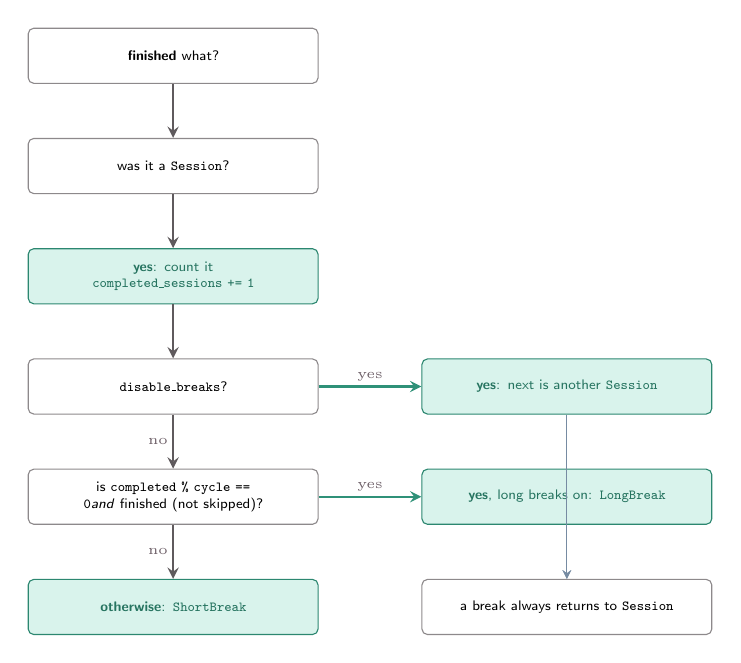
\begin{tikzpicture}[
  q/.style={rounded corners=2pt,draw=ink!50,fill=white,align=center,inner sep=4pt,
            font=\tiny\sffamily,minimum height=7mm,text width=34mm},
  yesb/.style={q,draw=mint!70!black,fill=mint!20,text=mint!60!black},
  n/.style={q,draw=accent!60,fill=accent!10,text=accent!55!black},
]
  \node[q] (a) at (0,0) {\textbf{finished} what?};
  \node[q] (b) at (0,-1.4) {was it a \texttt{Session}?};
  \node[yesb] (c) at (0,-2.8) {\textbf{yes}: count it\\\texttt{completed\_sessions += 1}};
  \node[q] (d) at (0,-4.2) {\texttt{disable\_breaks}?};
  \node[yesb] (e) at (5.0,-4.2) {\textbf{yes}: next is another \texttt{Session}};
  \node[q] (f) at (0,-5.6) {is \texttt{completed \% cycle == 0}\emph{and} finished (not skipped)?};
  \node[yesb] (g) at (5.0,-5.6) {\textbf{yes}, long breaks on: \texttt{LongBreak}};
  \node[yesb] (h) at (0,-7.0) {\textbf{otherwise}: \texttt{ShortBreak}};
  \node[q] (i) at (5.0,-7.0) {a break always returns to \texttt{Session}};

  \draw[e] (a)--(b); \draw[e] (b)--(c); \draw[e] (c)--(d);
  \draw[es] (d) -- node[vlabel, above, font=\tiny] {yes} (e);
  \draw[e] (d) -- node[vlabel, left, font=\tiny] {no} (f);
  \draw[es] (f) -- node[vlabel, above, font=\tiny] {yes} (g);
  \draw[e] (f) -- node[vlabel, left, font=\tiny] {no} (h);
  \draw[ethin, pastel!70!black] (e) -- (i);
  \draw[ethin, pastel!70!black] (g) -- (i);
\end{tikzpicture}
\caption{The decision tree of \texttt{advance()}. The highlighted boxes are the only
places in the whole codebase where the answer to ``what comes next?'' is decided.}
\label{fig:advance}
\end{figure}

\keybox{accent}{%
\textbf{The subtle line.} \code{due\_long} requires \code{completion == Completion::Finished}.
If the user skips a session that happens to land on a cycle boundary, the long break is
\emph{not} scheduled --- and \code{completed\_sessions} is not incremented either, so the
cycle counter stays aligned. The test \code{skipped\_session\_at\_cycle\_boundary\_does\_not\_schedule\_long\_break}
in \file{timer.rs} exists precisely to pin this down.}
\clearpage
\section{The Pomodoro cycle, end to end}

\subsection{Normal case: a 4-session cycle}

\begin{figure}[H]
\centering
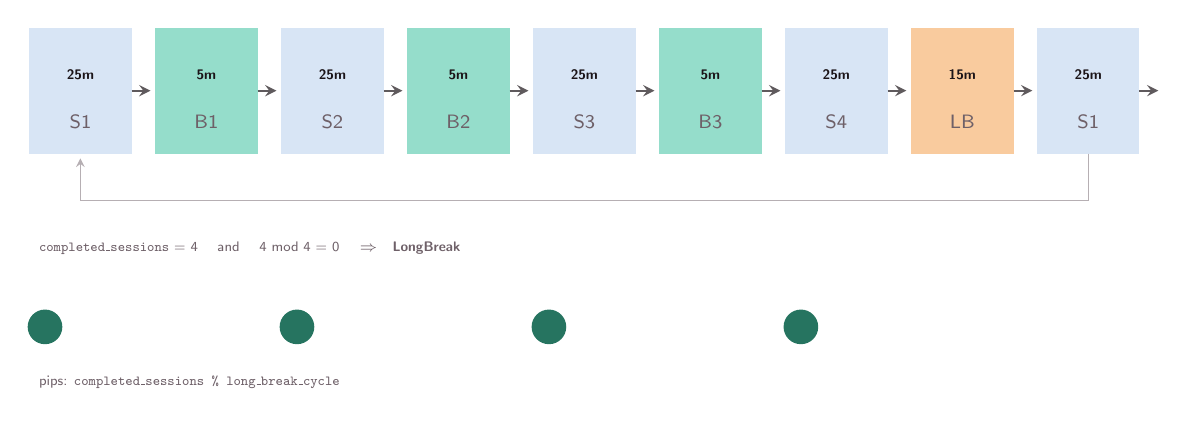
\begin{tikzpicture}[x=1mm,y=1mm]
  % nine blocks: S B S B S B S B LB
  \foreach \i/\lab/\col/\txt in {
    0/S1/pastel!45/{25m},
    1/B1/mint!55/{5m},
    2/S2/pastel!45/{25m},
    3/B2/mint!55/{5m},
    4/S3/pastel!45/{25m},
    5/B3/mint!55/{5m},
    6/S4/pastel!45/{25m},
    7/LB/mandarin!45/{15m},
    8/S1/pastel!45/{25m}}
  {
    \pgfmathsetmacro{\x}{\i*16}
    \fill[\col] (\x,30) rectangle ++(13,16);
    \node[anchor=center,font=\tiny\sffamily\bfseries,text=ink] at ({\x+6.5},40) {\txt};
    \node[anchor=center,font=\scriptsize\sffamily,text=softink] at ({\x+6.5},34) {\lab};
    \draw[e] ({\x+13},38) -- ({\x+15.4},38);
  }
  % the cycle wraps
  \draw[ethin, softink!50] (8*16+6.5,30) -- (8*16+6.5,24) -- (6.5,24) -- (6.5,29.4);
  \node[anchor=west,font=\tiny\sffamily,text=softink] at (0,18)
    {\texttt{completed\_sessions} = 4 \quad and \quad 4 mod 4 = 0 \quad$\Rightarrow$\quad \textbf{LongBreak}};
  % pips
  \foreach \i in {0,1,2,3} {
    \fill[mint!60!black] ({2+\i*32},8) circle (2.2);
  }
  \node[anchor=west,font=\tiny\sffamily,text=softink] at (0,1)
    {pips: \texttt{completed\_sessions \% long\_break\_cycle}};
\end{tikzpicture}
\caption{With the default settings (\texttt{long\_break\_cycle = 4}) the fourth finished
session earns a long break. Skipping any session breaks the chain --- the counter is
only incremented by \texttt{Completion::Finished}.}
\label{fig:cycle}
\end{figure}

\subsection{The three switches that reshape the cycle}

\begin{figure}[H]
\centering
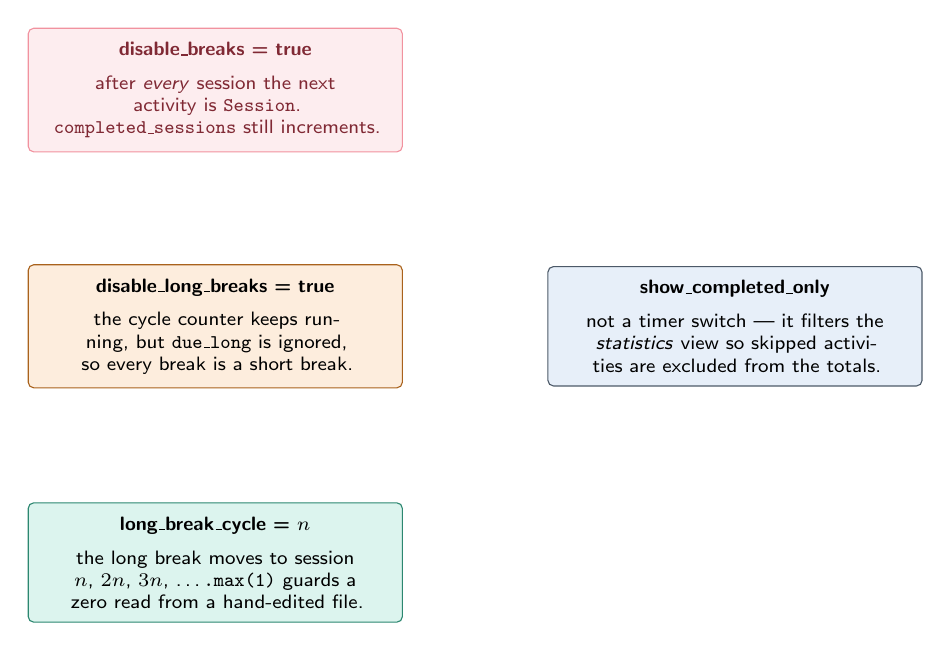
\begin{tikzpicture}[
  sw/.style={rounded corners=2pt,draw=ink!50,fill=white,align=center,inner sep=5pt,
             font=\scriptsize\sffamily,text width=44mm,minimum height=12mm},
]
  \node[sw, draw=accent!60, fill=accent!10, text=accent!55!black] (d1) at (0,0)
    {\textbf{disable\_breaks = true}\\[1.5mm]{\scriptsize after \emph{every} session the next\\activity is
     \texttt{Session}. \texttt{completed\_sessions} still increments.}};

  \node[sw, draw=mandarin!70!black, fill=mandarin!16] (d2) at (0,-3.0)
    {\textbf{disable\_long\_breaks = true}\\[1.5mm]{\scriptsize the cycle counter keeps running, but
     \texttt{due\_long} is ignored, so every break is a short break.}};

  \node[sw, draw=mint!70!black, fill=mint!18] (d3) at (0,-6.0)
    {\textbf{long\_break\_cycle = $n$}\\[1.5mm]{\scriptsize the long break moves to session $n$, $2n$,
     $3n$, \dots \texttt{.max(1)} guards a zero read from a hand-edited file.}};

  \node[sw, draw=pastel!45!black, fill=corefill] (d4) at (6.6,-3.0)
    {\textbf{show\_completed\_only}\\[1.5mm]{\scriptsize not a timer switch --- it filters the
     \emph{statistics} view so skipped activities are excluded from the totals.}};
\end{tikzpicture}
\caption{Four settings that change the shape of the cycle. The first three are read
inside \texttt{advance()} on every transition; the fourth only affects the numbers shown
in the statistics panel.}
\label{fig:switches}
\end{figure}

\subsection{Auto-start, and who decides it}

\begin{lstlisting}[caption={\file{app.rs}, \texttt{complete\_current()}. Note that the
core decides \emph{whether} to start the next activity, but never starts it itself
unless asked.}]
pub fn complete_current(&mut self) {
    let finished = self.timer.activity();
    self.status = format!("{} finished", finished.label());
    self.record(true);                       // write the CSV row first
    self.timer.finish();                     // advance; state becomes Idle
    self.notified = false;
    let auto = if self.timer.activity().is_break() {   // note: the NEXT activity
        self.settings.auto_start_break
    } else {
        self.settings.auto_start_session
    };
    if auto { self.timer.start(); }
}
\end{lstlisting}

\begin{figure}[H]
\centering
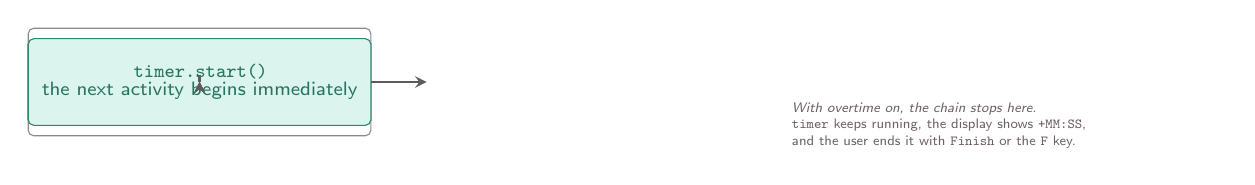
\begin{tikzpicture}[
  b/.style={rounded corners=2pt,draw=ink!50,fill=white,align=center,inner sep=5pt,
            font=\scriptsize\sffamily,text width=40mm,minimum height=11mm},
  k/.style={b,draw=accent!65,fill=accent!12,text=accent!55!black},
  g/.style={b,draw=mint!70!black,fill=mint!18,text=mint!60!black},
]
  \node[b] (t) {the displayed second\\reaches zero};
  \node[k] (n) {\texttt{tick()} raises\\\texttt{notify\_requested} \emph{once}};
  \node[b] (o) {\textbf{unless} \texttt{overtime},\\\texttt{complete\_current()}};
  \node[b] (s) {look up\\\texttt{auto\_start\_break}\\\emph{or}\\\texttt{auto\_start\_session}};
  \node[g] (st) {\texttt{timer.start()}\\[-0.5mm]{\scriptsize the next activity begins immediately}};

  \draw[e] (t)--(n); \draw[e] (n)--(o); \draw[e] (o)--(s); \draw[e] (s)--(st);
  \draw[e] (o.east) -- ++(7mm,0);
  \node[note, anchor=west, text width=54mm, align=left, font=\tiny\sffamily] at (7.4,-0.55)
    {\emph{With overtime on, the chain stops here.}\\
     \texttt{timer} keeps running, the display shows \texttt{+MM:SS},\\
     and the user ends it with \texttt{Finish} or the \texttt{F} key.};
\end{tikzpicture}
\caption{End-of-activity path with overtime off. With \texttt{overtime} on, the
completion is deferred and the activity stays running past zero.}
\label{fig:finishpath}
\end{figure}

\subsection{Overtime: the display flips sign}

\begin{lstlisting}[caption={\file{app.rs}. Overtime is a \emph{display} mode plus a
deferred completion; the timer itself never changes state.}]
pub fn display_seconds(&self) -> u64 {
    if self.is_overtime() {
        self.timer.elapsed().saturating_sub(self.timer.duration()).as_secs()
    } else {
        self.timer.remaining_display().as_secs()
    }
}
pub fn is_overtime(&self) -> bool {
    self.settings.overtime
        && self.timer.remaining().is_zero()
        && self.timer.state() != RunState::Idle
}
\end{lstlisting}

\begin{figure}[H]
\centering
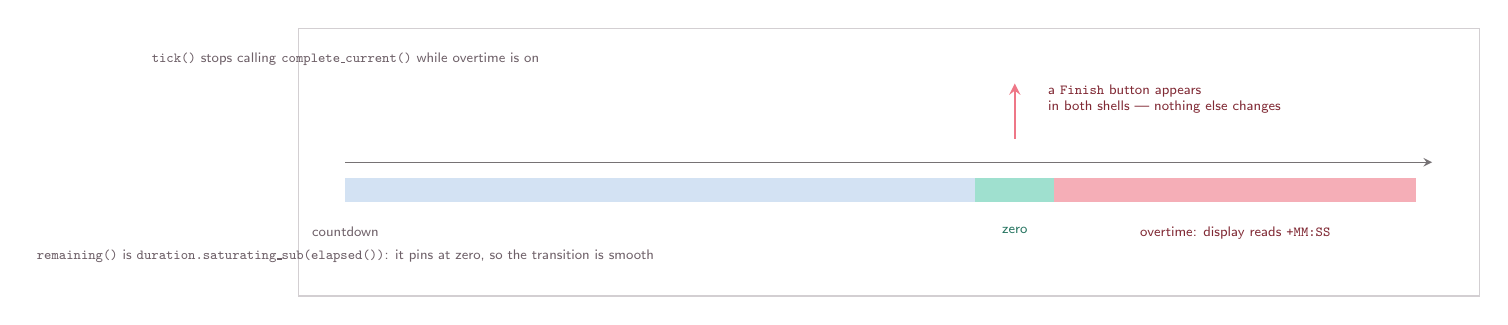
\begin{tikzpicture}[x=1mm,y=1mm]
  \draw[draw=softink!30,line width=0.5pt] (0,0) rectangle (150,34);
  \draw[-stealth, draw=ink!60] (6,17) -- (144,17);
  \fill[pastel!50] (6,12) rectangle (86,15);
  \fill[mint!50] (86,12) rectangle (96,15);
  \fill[accent!45] (96,12) rectangle (142,15);
  \node[anchor=north,font=\tiny\sffamily,text=softink] at (6,10) {countdown};
  \node[anchor=north,font=\tiny\sffamily,text=mint!60!black] at (91,10) {zero};
  \node[anchor=north,font=\tiny\sffamily,text=accent!55!black] at (119,10) {overtime: display reads \texttt{+MM:SS}};
  \node[anchor=south,font=\tiny\sffamily,text=softink] at (6,28)
    {\texttt{tick()} stops calling \texttt{complete\_current()} while overtime is on};
  \draw[er] (91,20) -- (91,27);
  \node[anchor=west,align=left,font=\tiny\sffamily,text=accent!55!black] at (94,25)
    {a \texttt{Finish} button appears\\in both shells --- nothing else changes};
  \node[anchor=south,font=\tiny\sffamily,text=softink] at (6,3)
    {\texttt{remaining()} is \texttt{duration.saturating\_sub(elapsed())}: it pins at zero, so the
     transition is smooth};
\end{tikzpicture}
\caption{Overtime is a display convention, not a fourth \texttt{RunState}.}
\label{fig:overtime}
\end{figure}
\clearpage
\section{The clock, and the display it feeds}

\subsection{Two clocks behind one type name}

\file{timer.rs} defines a private \texttt{Clock} enum with one variant per platform.
This is the only piece of the core that is platform-conditional, and it is 40 lines.

\begin{lstlisting}[caption={\file{timer.rs} lines 4--59, abridged.}]
#[derive(Clone, Copy, Debug)]
struct Clock {
    #[cfg(target_os = "macos")]      ticks:  u64,              // mach_continuous_time
    #[cfg(not(target_os = "macos"))] instant: std::time::Instant,
}
impl Clock {
    fn now() -> Self { /* one branch per platform */ }
    fn elapsed(self) -> Duration {
        #[cfg(target_os = "macos")]
        {
            static SCALE: OnceLock<(u32,u32)> = OnceLock::new();
            let &(numer, denom) = SCALE.get_or_init(|| { /* mach_timebase_info */ });
            let nanos = (Clock::now().ticks - self.ticks) as u128 * numer as u128
                        / denom as u128;
            Duration::from_nanos(nanos.min(u64::MAX as u128) as u64)
        }
        #[cfg(not(target_os = "macos"))]
        { self.instant.elapsed() }
    }
}
unsafe extern "C" { fn mach_continuous_time() -> u64; fn mach_timebase_info(..) -> i32; }
\end{lstlisting}

\begin{figure}[H]
\centering
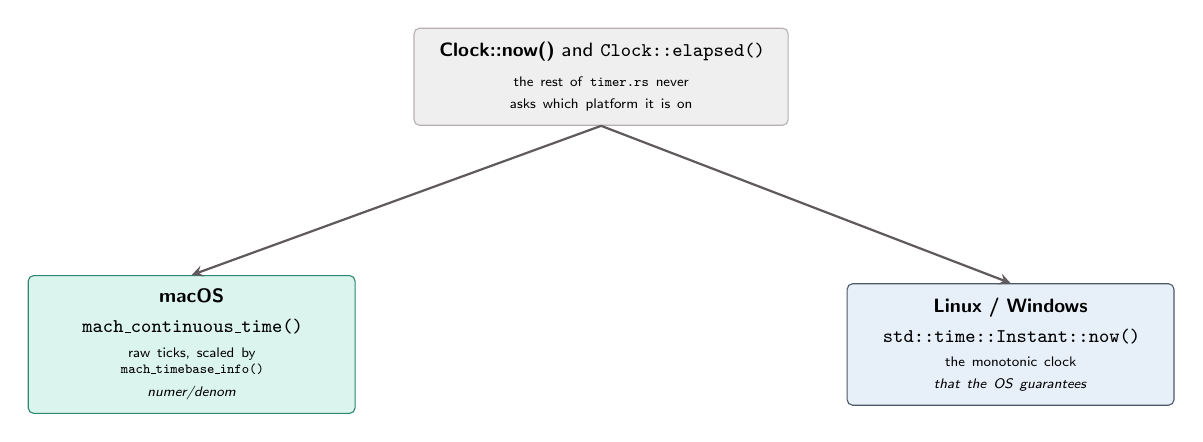
\begin{tikzpicture}[
  c/.style={rounded corners=2pt,draw=ink!50,fill=white,align=center,inner sep=5pt,
            font=\scriptsize\sffamily,text width=38mm,minimum height=12mm},
  mac/.style={c,draw=mint!70!black,fill=mint!18},
  oth/.style={c,draw=pastel!45!black,fill=corefill},
]
  \node[c, draw=softink!50, fill=soft, text width=44mm] (api) at (0,0)
    {\textbf{Clock::now()} and \texttt{Clock::elapsed()}\\[1mm]
     {\tiny the rest of \texttt{timer.rs} never asks which platform it is on}};

  \node[mac] (m) at (-5.2,-3.4) {\textbf{macOS}\\[1mm]\texttt{mach\_continuous\_time()}\\[1mm]
     {\tiny raw ticks, scaled by\\\texttt{mach\_timebase\_info()}\\\textit{numer/denom}}};
  \node[oth] (o) at (5.2,-3.4) {\textbf{Linux / Windows}\\[1mm]\texttt{std::time::Instant::now()}\\[1mm]
     {\tiny the monotonic clock\\\textit{that the OS guarantees}}};
  \draw[e] (api.south) -- (m.north);
  \draw[e] (api.south) -- (o.north);
\end{tikzpicture}
\caption{\texttt{Clock} is the entire platform abstraction of the core.}
\label{fig:clock}
\end{figure}

\keybox{mint}{\textbf{Why \code{mach\_continuous\_time} and not
\code{mach\_absolute\_time}?} The ``continuous'' variant keeps counting while the
machine is asleep, which is what a Pomodoro timer wants: if the lid is shut for ten
minutes, the session really did advance by ten minutes and
\texttt{App::sleep()} decides separately whether to pause it. The timebase
conversion is cached in a \code{OnceLock} because it is a constant for the lifetime
of the process.}

\subsection{Rounding: why a fresh timer shows 25:00, not 24:59}

Two tiny functions carry all of the display logic, and both exist because the
alternative was a visible one-second jitter.

\begin{lstlisting}[caption={Round up, so the label is stable for a whole second.},basicstyle=\ttfamily\footnotesize]
pub fn remaining\_display(\&self) -> Duration {
    let remaining = self.remaining();
    if remaining.is_zero() { return Duration::ZERO; }
    Duration::from_secs(remaining.as_secs() + u64::from(remaining.subsec_nanos() != 0))
}
\end{lstlisting}

\begin{lstlisting}[caption={Sleep exactly until the label would change --- not,basicstyle=\ttfamily\footnotesize],basicstyle=\ttfamily\footnotesize],basicstyle=\ttfamily\footnotesize],basicstyle=\ttfamily\footnotesize],basicstyle=\ttfamily\footnotesize],basicstyle=\ttfamily\footnotesize],basicstyle=\ttfamily\footnotesize],basicstyle=\ttfamily\footnotesize],basicstyle=\ttfamily\footnotesize],basicstyle=\ttfamily\footnotesize],basicstyle=\ttfamily\footnotesize],basicstyle=\ttfamily\footnotesize],basicstyle=\ttfamily\footnotesize],basicstyle=\ttfamily\footnotesize],basicstyle=\ttfamily\footnotesize],basicstyle=\ttfamily\footnotesize],basicstyle=\ttfamily\footnotesize],basicstyle=\ttfamily\footnotesize],basicstyle=\ttfamily\footnotesize],basicstyle=\ttfamily\footnotesize],basicstyle=\ttfamily\footnotesize],basicstyle=\ttfamily\footnotesize],basicstyle=\ttfamily\footnotesize],basicstyle=\ttfamily\footnotesize],basicstyle=\ttfamily\footnotesize],basicstyle=\ttfamily\footnotesize],basicstyle=\ttfamily\footnotesize],basicstyle=\ttfamily\footnotesize],basicstyle=\ttfamily\footnotesize],basicstyle=\ttfamily\footnotesize],basicstyle=\ttfamily\footnotesize],basicstyle=\ttfamily\footnotesize],basicstyle=\ttfamily\footnotesize],basicstyle=\ttfamily\footnotesize],basicstyle=\ttfamily\footnotesize],basicstyle=\ttfamily\footnotesize],basicstyle=\ttfamily\footnotesize],basicstyle=\ttfamily\footnotesize],basicstyle=\ttfamily\footnotesize],basicstyle=\ttfamily\footnotesize],basicstyle=\ttfamily\footnotesize],basicstyle=\ttfamily\footnotesize],basicstyle=\ttfamily\footnotesize],basicstyle=\ttfamily\footnotesize],basicstyle=\ttfamily\footnotesize],basicstyle=\ttfamily\footnotesize],basicstyle=\ttfamily\footnotesize],basicstyle=\ttfamily\footnotesize],basicstyle=\ttfamily\footnotesize],basicstyle=\ttfamily\footnotesize],basicstyle=\ttfamily\footnotesize],basicstyle=\ttfamily\footnotesize],basicstyle=\ttfamily\footnotesize],basicstyle=\ttfamily\footnotesize],basicstyle=\ttfamily\footnotesize],basicstyle=\ttfamily\footnotesize],basicstyle=\ttfamily\footnotesize],basicstyle=\ttfamily\footnotesize],basicstyle=\ttfamily\footnotesize],basicstyle=\ttfamily\footnotesize],basicstyle=\ttfamily\footnotesize],basicstyle=\ttfamily\footnotesize],basicstyle=\ttfamily\footnotesize],basicstyle=\ttfamily\footnotesize],basicstyle=\ttfamily\footnotesize],basicstyle=\ttfamily\footnotesize],basicstyle=\ttfamily\footnotesize],basicstyle=\ttfamily\footnotesize],basicstyle=\ttfamily\footnotesize],basicstyle=\ttfamily\footnotesize],basicstyle=\ttfamily\footnotesize],basicstyle=\ttfamily\footnotesize],basicstyle=\ttfamily\footnotesize],basicstyle=\ttfamily\footnotesize],basicstyle=\ttfamily\footnotesize],basicstyle=\ttfamily\footnotesize],basicstyle=\ttfamily\footnotesize],basicstyle=\ttfamily\footnotesize],basicstyle=\ttfamily\footnotesize],basicstyle=\ttfamily\footnotesize],basicstyle=\ttfamily\footnotesize],basicstyle=\ttfamily\footnotesize],basicstyle=\ttfamily\footnotesize],basicstyle=\ttfamily\footnotesize],basicstyle=\ttfamily\footnotesize],basicstyle=\ttfamily\footnotesize],basicstyle=\ttfamily\footnotesize],basicstyle=\ttfamily\footnotesize],basicstyle=\ttfamily\footnotesize],basicstyle=\ttfamily\footnotesize],basicstyle=\ttfamily\footnotesize],basicstyle=\ttfamily\footnotesize],basicstyle=\ttfamily\footnotesize],basicstyle=\ttfamily\footnotesize],basicstyle=\ttfamily\footnotesize],basicstyle=\ttfamily\footnotesize],basicstyle=\ttfamily\footnotesize],basicstyle=\ttfamily\footnotesize],basicstyle=\ttfamily\footnotesize],basicstyle=\ttfamily\footnotesize],basicstyle=\ttfamily\footnotesize],basicstyle=\ttfamily\footnotesize],basicstyle=\ttfamily\footnotesize],basicstyle=\ttfamily\footnotesize],basicstyle=\ttfamily\footnotesize],basicstyle=\ttfamily\footnotesize],basicstyle=\ttfamily\footnotesize],basicstyle=\ttfamily\footnotesize],basicstyle=\ttfamily\footnotesize],basicstyle=\ttfamily\footnotesize],basicstyle=\ttfamily\footnotesize],basicstyle=\ttfamily\footnotesize],basicstyle=\ttfamily\footnotesize],basicstyle=\ttfamily\footnotesize],basicstyle=\ttfamily\footnotesize],basicstyle=\ttfamily\footnotesize],basicstyle=\ttfamily\footnotesize],basicstyle=\ttfamily\footnotesize],basicstyle=\ttfamily\footnotesize],basicstyle=\ttfamily\footnotesize],basicstyle=\ttfamily\footnotesize],basicstyle=\ttfamily\footnotesize],basicstyle=\ttfamily\footnotesize],basicstyle=\ttfamily\footnotesize],basicstyle=\ttfamily\footnotesize],basicstyle=\ttfamily\footnotesize],basicstyle=\ttfamily\footnotesize]
\texttt{duration - remaining}, the complement, and busy.}]
pub fn next_display_change(&self) -> Duration {
    let remaining = self.remaining();
    if remaining.is_zero() { return Duration::from_secs(1); }
    let nanos = remaining.subsec_nanos();
    if nanos == 0 { Duration::from_secs(1) } else { Duration::from_nanos(u64::from(nanos)) }
}
\end{lstlisting}

\begin{figure}[H]
\centering
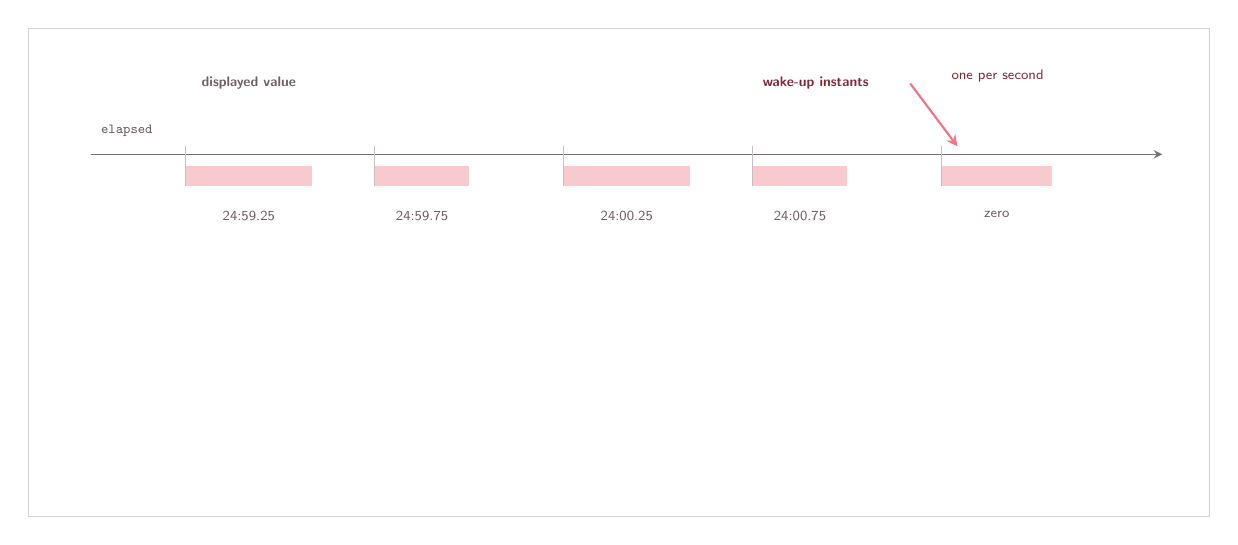
\begin{tikzpicture}[x=1mm,y=1mm]
  \draw[draw=softink!30,line width=0.5pt] (0,0) rectangle (150,62);
  % timeline
  \draw[-stealth, draw=ink!60] (8,46) -- (144,46);
  \node[anchor=south west,font=\tiny\sffamily,text=softink] at (8,47) {\texttt{elapsed}};

  % sub-second slivers
  \foreach \fx/\fw/\flab in {20/16/{24:59.25}, 44/12/{24:59.75}, 68/16/{24:00.25}, 92/12/{24:00.75}, 116/14/{zero}}
  {
    \fill[accent!30] (\fx,42) rectangle ({\fx+\fw},44.5);
    \draw[softink!40] (\fx,42) -- (\fx,47);
    \node[anchor=north,font=\tiny\sffamily,text=softink,align=center] at ({\fx+\fw/2},40) {\flab};
  }
  % labels
  \node[anchor=south,font=\tiny\sffamily\bfseries,text=softink] at (28,53) {displayed value};
  \node[anchor=south,font=\tiny\sffamily\bfseries,text=accent!55!black] at (100,53) {wake-up instants};
  \node[anchor=west,font=\tiny\sffamily,text=accent!55!black] at (116,56) {one per second};
  \draw[er] (112,55) -- (118,47);

  \end{tikzpicture}
\end{figure}

\begin{center}\small
\begin{minipage}{0.92\linewidth}
\texttt{remaining\_display()} rounds \emph{up}: with $0.25$\,s left the label still
prints \texttt{24:59}, so it changes exactly when the fractional part reaches zero.

\texttt{next\_display\_change()} returns the \emph{complement} of that, i.e.\ the time
\emph{until} the boundary --- $0.75$\,s at the first sample above, not $0.25$\,s.
\end{minipage}
\end{center}

\begin{figure}[H]
\centering
\caption{The two functions exist to keep each other honest: round up for the label, and
sleep until the label would change.}
\label{fig:rounding}
\end{figure}

\subsection{How each shell spends that delay}

\begin{table}[H]
\centering\small
\begin{tabular}{@{}p{30mm} p{66mm} p{62mm}@{}}
\toprule
& \textbf{mac\_shell.rs} & \textbf{egui\_shell.rs} \\
\midrule
Idle timer & no timer armed & no repaint scheduled \\
Running & \texttt{refresh()} ends with a one-shot \texttt{NSTimer} &
\texttt{schedule\_repaint()} calls \texttt{ctx.request\_repaint\_after(d)} \\
Tolerance & \texttt{setTolerance(0.02)} --- the OS may fire 20\,ms late &
exact; egui coalesces into the next frame \\
Clamped to & $\max(0.01\,\text{s})$ & n/a \\
Repeat? & \texttt{repeats: false}, then re-armed in \texttt{refresh()} & re-armed every frame \\
\bottomrule
\end{tabular}
\caption{Both shells converge on the same rule: schedule exactly one wake-up, at the
next visible change. Neither one ever busy-waits.}
\end{table}

\begin{lstlisting}[caption={\file{app.rs} lines 172--176: the whole scheduling policy is
three lines.}]
#[cfg(feature = "egui-ui")]
pub fn schedule_repaint(&self, ctx: &egui::Context) {
    if self.timer.state() == RunState::Running {
        ctx.request_repaint_after(self.timer.next_display_change());
    }
}
\end{lstlisting}

\begin{figure}[H]
\centering
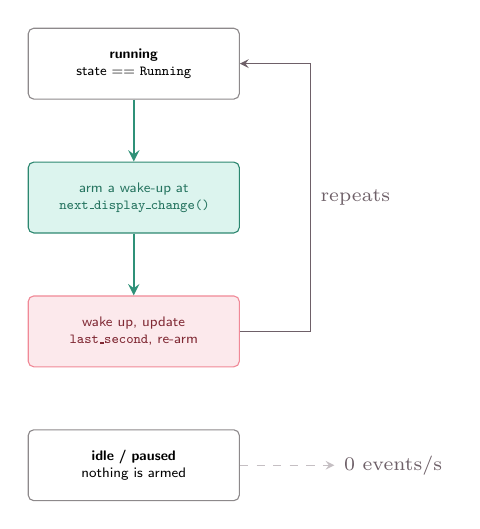
\begin{tikzpicture}[
  b/.style={rounded corners=2pt,draw=ink!50,fill=white,align=center,inner sep=4pt,
            font=\tiny\sffamily,text width=24mm,minimum height=9mm},
  k/.style={b,draw=accent!65,fill=accent!12,text=accent!55!black},
  g/.style={b,draw=mint!70!black,fill=mint!18,text=mint!60!black},
]
  \node[b] (a) at (0,0) {\textbf{running}\\{\tiny state == \texttt{Running}}};
  \node[g] (b) at (0,-1.7) {\tiny arm a wake-up at\\\texttt{next\_display\_change()}};
  \node[k] (c) at (0,-3.4) {\tiny wake up, update\\\texttt{last\_second}, re-arm};
  \node[b] (d) at (0,-5.1) {\textbf{idle / paused}\\{\tiny nothing is armed}};
  \draw[es] (a)--(b); \draw[es] (b)--(c);
  \draw[ethin, softink] (c.east) -- ++(9mm,0) |- (a.east) node[pos=0.25,right,font=\tiny,text=softink] {\scriptsize repeats};
  \draw[ethin, softink!40, dashed] (d.east) -- ++(12mm,0) node[right,font=\tiny,text=softink] {\scriptsize 0 events/s};
\end{tikzpicture}
\caption{The repaint loop, which is really just a one-node cycle.}
\label{fig:repaint}
\end{figure}
\clearpage
\section{The intent-flag pattern, in full}

This is the pattern that makes the whole project work, so it is worth seeing every
place it is used. There are exactly five flags, and each one has a producer in the core
and a consumer in the shell.

\subsection{The five flags, their producers, their consumers}

\begin{figure}[H]
\centering
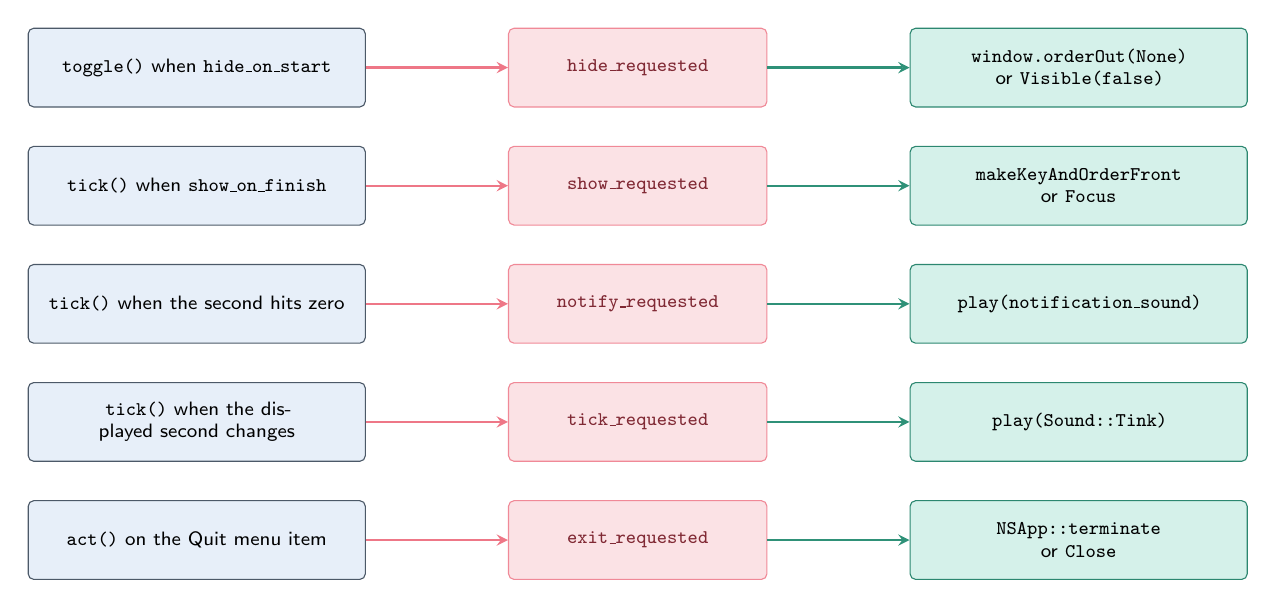
\begin{tikzpicture}[
  fl/.style={rounded corners=2pt,draw=accent!65,fill=intentfill,align=center,inner sep=4pt,
             font=\scriptsize\sffamily,text width=30mm,minimum height=10mm,
             text=accent!55!black},
  pr/.style={rounded corners=2pt,draw=pastel!45!black,fill=corefill,align=center,inner sep=4pt,
             font=\scriptsize\sffamily,text width=40mm,minimum height=10mm},
  co/.style={rounded corners=2pt,draw=mint!70!black,fill=shellfill,align=center,inner sep=4pt,
             font=\scriptsize\sffamily,text width=40mm,minimum height=10mm},
]
  \node[fl] (f1) at (0,0) {\texttt{hide\_requested}};
  \node[fl] (f2) at (0,-1.5) {\texttt{show\_requested}};
  \node[fl] (f3) at (0,-3.0) {\texttt{notify\_requested}};
  \node[fl] (f4) at (0,-4.5) {\texttt{tick\_requested}};
  \node[fl] (f5) at (0,-6.0) {\texttt{exit\_requested}};

  \node[pr] (p1) at (-5.6,0) {\texttt{toggle()} when \texttt{hide\_on\_start}};
  \node[pr] (p2) at (-5.6,-1.5) {\texttt{tick()} when \texttt{show\_on\_finish}};
  \node[pr] (p3) at (-5.6,-3.0) {\texttt{tick()} when the second hits zero};
  \node[pr] (p4) at (-5.6,-4.5) {\texttt{tick()} when the displayed second changes};
  \node[pr] (p5) at (-5.6,-6.0) {\texttt{act()} on the Quit menu item};

  \node[co] (c1) at (5.6,0) {\texttt{window.orderOut(None)}\\\scriptsize or \texttt{Visible(false)}};
  \node[co] (c2) at (5.6,-1.5) {\texttt{makeKeyAndOrderFront}\\\scriptsize or \texttt{Focus}};
  \node[co] (c3) at (5.6,-3.0) {\texttt{play(notification\_sound)}};
  \node[co] (c4) at (5.6,-4.5) {\texttt{play(Sound::Tink)}};
  \node[co] (c5) at (5.6,-6.0) {\texttt{NSApp::terminate}\\\scriptsize or \texttt{Close}};

  \foreach \i in {1,2,3,4,5} {
    \draw[er] (p\i.east) -- (f\i.west);
    \draw[es] (f\i.east) -- (c\i.west);
  }
\end{tikzpicture}
\caption{Every flag is a one-way trip: the core sets it, the shell reads-and-clears it.
There is no callback, no closure, no channel, and no shared mutable state beyond the
flag itself.}
\label{fig:flags}
\end{figure}

\subsection{Why \texttt{mem::take} and not \texttt{if}}

\begin{figure}[H]
\centering
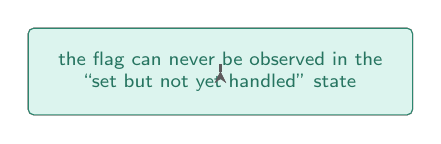
\begin{tikzpicture}[
  b/.style={rounded corners=2pt,draw=ink!50,fill=white,align=center,inner sep=4pt,
            font=\scriptsize\sffamily,text width=46mm,minimum height=11mm},
  k/.style={b,draw=accent!65,fill=accent!12,text=accent!55!black},
  g/.style={b,draw=mint!70!black,fill=mint!18,text=mint!60!black},
]
  \node[b] (a) {\textbf{the naive version}\\[1mm]{\scriptsize test, then write, then branch}};
  \node[k] (b) {\textbf{\texttt{mem::take}}\\[1mm]{\scriptsize one read, one write, one branch}};
  \node[g] (c) {the flag can never be observed in the\\``set but not yet handled'' state};
  \draw[e] (a)--(b); \draw[e] (b)--(c);
\end{tikzpicture}
\caption{\texttt{std::mem::take} replaces the value with \texttt{Default::default()} and
returns the old one, so the test and the reset are a single operation.}
\label{fig:memtake}
\end{figure}

\begin{lstlisting}[caption={The two versions side by side. The second is what both shells use.}]
// naive: two steps, and a window in between
if app.notify_requested {
    play(sound);
    app.notify_requested = false;
}

// mem::take: one step, no window
if std::mem::take(&mut app.notify_requested) {
    play(sound);
}
\end{lstlisting}

\subsection{The one flag that is not a flag}

\texttt{exit\_requested} is set by the shell itself (the Quit menu item calls
\texttt{NSApplication::terminate} directly in the AppKit shell), so it is the only one
whose producer is not the core. Everything else follows the rule.

\subsection{Sleep and wake}

\begin{figure}[H]
\centering
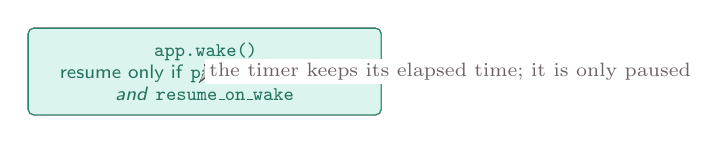
\begin{tikzpicture}[
  b/.style={rounded corners=2pt,draw=ink!50,fill=white,align=center,inner sep=4pt,
            font=\scriptsize\sffamily,text width=42mm,minimum height=11mm},
  k/.style={b,draw=accent!65,fill=accent!12,text=accent!55!black},
  g/.style={b,draw=mint!70!black,fill=mint!18,text=mint!60!black},
]
  \node[b] (a) {\textbf{macOS will sleep}};
  \node[k] (b) {\texttt{app.sleep()}\\\scriptsize \texttt{pause\_on\_start} \emph{and} Running};
  \node[b] (c) {\texttt{timer.pause()}\\\texttt{paused\_for\_sleep = true}};
  \node[b] (d) {\textbf{macOS wakes}};
  \node[g] (e) {\texttt{app.wake()}\\\scriptsize resume only if \texttt{paused\_for\_sleep}\\\emph{and} \texttt{resume\_on\_wake}};
  \draw[e] (a)--(b); \draw[e] (b)--(c);
  \draw[e] (d)--(e);
  \draw[ethin, softink!40, dashed] (c) -- node[vlabel, right, font=\tiny, text=softink]
    {\scriptsize the timer keeps its elapsed time; it is only paused} (e);
\end{tikzpicture}
\caption{Sleep handling is a two-step handshake. The \texttt{paused\_for\_sleep} field is
what stops a wake from resuming a timer the user had paused themselves.}
\label{fig:sleep}
\end{figure}

\begin{lstlisting}[caption={\file{app.rs} lines 177--188. The asymmetry is the point.}]
pub fn sleep(&mut self) {
    if self.settings.pause_on_sleep && self.timer.state() == RunState::Running {
        self.timer.pause();
        self.paused_for_sleep = true;
    }
}
pub fn wake(&mut self) {
    if self.paused_for_sleep && self.settings.resume_on_wake { self.timer.start(); }
    self.paused_for_sleep = false;
}
\end{lstlisting}
\clearpage
\section{\texttt{tick()}: the one function that runs every second}

Everything the app does once a second goes through \texttt{App::tick()}. It is 23 lines
and it is the only place where the core decides that something has changed.

\begin{lstlisting}[caption={\file{app.rs} lines 133--155, complete.}]
pub fn tick(&mut self) {
    if self.timer.state() != RunState::Running { return; }        // (1) idle: do nothing
    if self.timer.remaining().is_zero() {                        // (2) the second hit zero
        if !self.notified {
            self.notified = true;
            self.notify_requested = true;
            if self.settings.show_on_finish { self.show_requested = true; }
        }
        if !self.settings.overtime { self.complete_current(); }  // (3) or keep running
    }
    let second = self.display_seconds();                         // (4) did the label change?
    if second != self.last_second {
        self.last_second = second;
        self.tick_requested = self.settings.ticking_sound
            && !(self.settings.mute_ticking_on_break && self.timer.activity().is_break());
    }
}
\end{lstlisting}

\subsection{The four decisions, in order}

\begin{figure}[H]
\centering
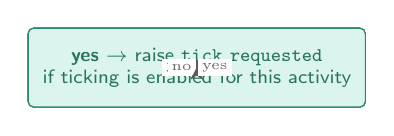
\begin{tikzpicture}[
  d/.style={rounded corners=2pt,draw=ink!50,fill=white,align=center,inner sep=4pt,
            font=\scriptsize\sffamily,text width=40mm,minimum height=10mm},
  yesb/.style={d,draw=mint!70!black,fill=mint!18,text=mint!60!black},
  n/.style={d,draw=accent!60,fill=accent!10,text=accent!55!black},
]
  \node[d] (s) {\textbf{(1)} is the timer Running?};
  \node[n] (r) {\textbf{no} $\rightarrow$ \texttt{return}\\\scriptsize nothing else runs};
  \node[d] (z) {\textbf{(2)} is \texttt{remaining()} zero?};
  \node[yesb] (nt) {\textbf{yes} $\rightarrow$ raise \texttt{notify\_requested}\\\scriptsize once, guarded by \texttt{notified}};
  \node[d] (ov) {\textbf{(3)} is \texttt{overtime} off?};
  \node[yesb] (cc) {\textbf{yes} $\rightarrow$ \texttt{complete\_current()}\\\scriptsize record, advance, maybe auto-start};
  \node[d] (ds) {\textbf{(4)} did \texttt{display\_seconds()} change?};
  \node[yesb] (tk) {\textbf{yes} $\rightarrow$ raise \texttt{tick\_requested}\\\scriptsize if ticking is enabled for this activity};

  \draw[e] (s) -- node[vlabel, right, font=\tiny] {no} (r);
  \draw[e] (s) -- node[vlabel, left, font=\tiny] {yes} (z);
  \draw[e] (z) -- node[vlabel, right, font=\tiny] {yes} (nt);
  \draw[e] (nt) -- (ov);
  \draw[e] (z) -- node[vlabel, left, font=\tiny] {no} (ds);
  \draw[e] (ov) -- node[vlabel, right, font=\tiny] {yes} (cc);
  \draw[e] (ov) -- node[vlabel, left, font=\tiny] {no} (ds);
  \draw[e] (cc) -- (ds);
  \draw[e] (ds) -- node[vlabel, right, font=\tiny] {yes} (tk);
\end{tikzpicture}
\caption{\texttt{tick()} as a decision tree. Note that step (4) runs even when the
activity just completed, so the tick sound and the completion sound cannot collide.}
\label{fig:ticktree}
\end{figure}

\subsection{The \texttt{notified} guard}

\begin{figure}[H]
\centering
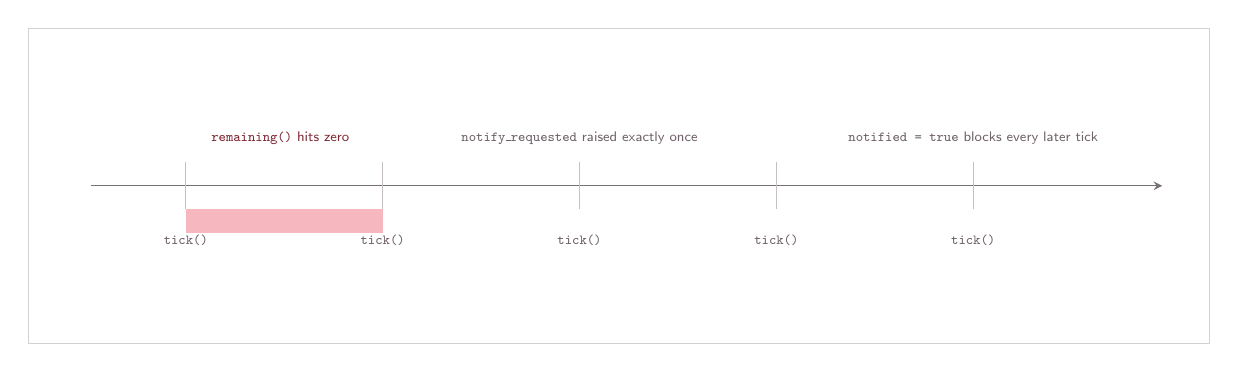
\begin{tikzpicture}[x=1mm,y=1mm]
  \draw[draw=softink!30,line width=0.5pt] (0,0) rectangle (150,40);
  \draw[-stealth, draw=ink!60] (8,20) -- (144,20);
  \foreach \x in {20,45,70,95,120} {
    \draw[softink!40] (\x,17) -- (\x,23);
    \node[anchor=north,font=\tiny\sffamily,text=softink] at (\x,15) {\texttt{tick()}};
  }
  \fill[accent!40] (20,14) rectangle (45,17);
  \node[anchor=south,font=\tiny\sffamily,text=accent!55!black] at (32,24)
    {\texttt{remaining()} hits zero};
  \node[anchor=south,font=\tiny\sffamily,text=softink] at (70,24)
    {\texttt{notify\_requested} raised exactly once};
  \node[anchor=south,font=\tiny\sffamily,text=softink] at (120,24)
    {\texttt{notified = true} blocks every later tick};
\end{tikzpicture}
\caption{Without the \texttt{notified} field, every subsequent tick would re-raise
\texttt{notify\_requested} and the shell would play the sound once per second forever.}
\label{fig:notified}
\end{figure}

\subsection{Recording an activity}

\begin{figure}[H]
\centering
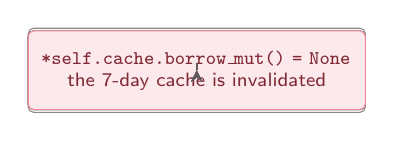
\begin{tikzpicture}[
  b/.style={rounded corners=2pt,draw=ink!50,fill=white,align=center,inner sep=4pt,
            font=\scriptsize\sffamily,text width=40mm,minimum height=10mm},
  k/.style={b,draw=accent!65,fill=accent!12,text=accent!55!black},
  g/.style={b,draw=mint!70!black,fill=mint!18,text=mint!60!black},
]
  \node[b] (a) {\texttt{record(completed)}\\\scriptsize called by \texttt{skip()} and \texttt{complete\_current()}};
  \node[b] (b) {\texttt{elapsed = timer.elapsed()}\\\scriptsize \emph{or} \texttt{duration} if completed};
  \node[g] (c) {\texttt{stats.record(activity, seconds, completed)}};
  \node[b] (d) {append one line to \texttt{activities.csv}};
  \node[k] (e) {\texttt{*self.cache.borrow\_mut() = None}\\\scriptsize the 7-day cache is invalidated};
  \draw[e] (a)--(b); \draw[e] (b)--(c); \draw[e] (c)--(d); \draw[e] (d)--(e);
\end{tikzpicture}
\caption{Recording is a single append plus a cache invalidation. There is no read-modify-write
of the file, so a crash cannot corrupt the log.}
\label{fig:record}
\end{figure}

\begin{lstlisting}[caption={\file{app.rs} lines 100--110. The \texttt{max} is what makes a
completed session count as a full session even if the user let it run into overtime.}]
fn record(&mut self, completed: bool) {
    let elapsed = self.timer.elapsed().as_secs();
    let seconds = if completed {
        elapsed.max(self.timer.duration().as_secs())
    } else {
        elapsed
    };
    if let Err(error) = self.stats.record(self.timer.activity(), seconds, completed) {
        self.status = format!("Activity save failed: {error}");
    }
}
\end{lstlisting}
\clearpage
\section{Persistence: two plain-text formats}

The app has no database, no serialization framework, and no \texttt{serde}. Both stores
are plain text with a hand-written parser, and both are written atomically.

\subsection{Where the files live}

\begin{figure}[H]
\centering
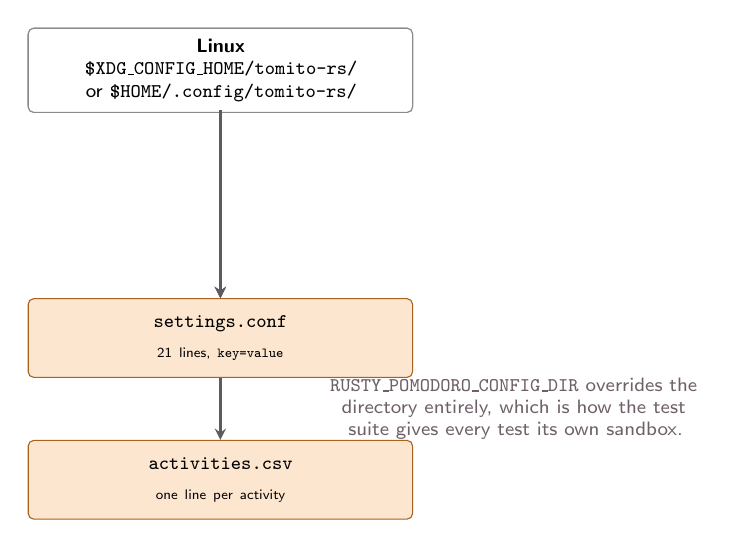
\begin{tikzpicture}[
  p/.style={rounded corners=2pt,draw=ink!50,fill=white,align=center,inner sep=4pt,
            font=\scriptsize\sffamily,text width=46mm,minimum height=10mm},
  d/.style={p,draw=mandarin!70!black,fill=datafill},
]
  \node[p] (mac) {\textbf{macOS}\\\texttt{\$HOME/Library/Application Support/tomito-rs/}};
  \node[p] (win) {\textbf{Windows}\\\texttt{\%APPDATA\%/tomito-rs/}};
  \node[p] (lin) {\textbf{Linux}\\\texttt{\$XDG\_CONFIG\_HOME/tomito-rs/} or \texttt{\$HOME/.config/tomito-rs/}};
  \node[d] (f1) at (0,-3.4) {\texttt{settings.conf}\\[1mm]{\tiny 21 lines, \texttt{key=value}}};
  \node[d] (f2) at (0,-5.2) {\texttt{activities.csv}\\[1mm]{\tiny one line per activity}};
  \draw[e] (mac.south) -- (f1.north);
  \draw[e] (win.south) -- (f1.north);
  \draw[e] (lin.south) -- (f1.north);
  \draw[e] (f1) -- (f2);
  \node[note, anchor=west, text width=52mm] at (1.0,-4.3)
    {\texttt{RUSTY\_POMODORO\_CONFIG\_DIR} overrides the directory entirely, which is how the
     test suite gives every test its own sandbox.};
\end{tikzpicture}
\caption{\file{config::config\_dir()} picks the platform directory. The override
environment variable is the only configuration the app reads at startup.}
\label{fig:paths}
\end{figure}

\subsection{\texttt{settings.conf}: write it, read it, clamp it}

\begin{figure}[H]
\centering
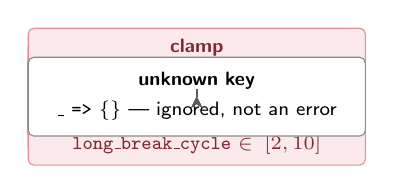
\begin{tikzpicture}[
  b/.style={rounded corners=2pt,draw=ink!50,fill=white,align=center,inner sep=4pt,
            font=\scriptsize\sffamily,text width=40mm,minimum height=10mm},
  k/.style={b,draw=accent!65,fill=accent!12,text=accent!55!black},
  g/.style={b,draw=mint!70!black,fill=mint!18,text=mint!60!black},
]
  \node[b] (a) {\textbf{serialize}\\[1mm]\texttt{writeln!(text, "{}=\{\}",\\   stringify!(\$field), self.\$field)}};
  \node[g] (b) {\textbf{save}\\[1mm]write to \texttt{settings.conf.tmp}\\\scriptsize then \texttt{fs::rename} into place};
  \node[b] (c) {\textbf{parse}\\[1mm]split on the first \texttt{=}, trim both sides};
  \node[k] (d) {\textbf{clamp}\\[1mm]\texttt{session\_minutes} $\in [1,180]$\\\texttt{short\_break\_minutes} $\in [1,60]$\\\texttt{long\_break\_minutes} $\in [1,120]$\\\texttt{long\_break\_cycle} $\in [2,10]$};
  \node[b] (e) {\textbf{unknown key}\\[1mm]\texttt{\_ => \{\}} --- ignored, not an error};
  \draw[e] (a)--(b); \draw[e] (b)--(c); \draw[e] (c)--(d); \draw[e] (d)--(e);
\end{tikzpicture}
\caption{The settings pipeline. Every numeric field is range-checked on read, so a
hand-edited file cannot produce a 9999-minute session.}
\label{fig:settings}
\end{figure}

\begin{table}[H]
\centering\small
\begin{tabular}{@{}p{40mm} p{30mm} p{70mm}@{}}
\toprule
\textbf{Field} & \textbf{Default} & \textbf{Notes} \\
\midrule
\texttt{session\_minutes} & 25 & clamped to 1--180 \\
\texttt{short\_break\_minutes} & 5 & clamped to 1--60 \\
\texttt{long\_break\_minutes} & 15 & clamped to 1--120 \\
\texttt{long\_break\_cycle} & 4 & clamped to 2--10 \\
\texttt{auto\_start\_session} & true & read by \texttt{complete\_current()} \\
\texttt{auto\_start\_break} & true & read by \texttt{complete\_current()} \\
\texttt{disable\_breaks} & false & read by \texttt{advance()} \\
\texttt{disable\_long\_breaks} & false & read by \texttt{advance()} \\
\texttt{show\_completed\_only} & true & filters the statistics view \\
\texttt{hide\_on\_start} & false & raises \texttt{hide\_requested} \\
\texttt{keep\_in\_front} & false & window level \\
\texttt{hide\_on\_launch} & false & applied once in \texttt{App::new} \\
\texttt{show\_on\_finish} & true & raises \texttt{show\_requested} \\
\texttt{overtime} & false & display mode + deferred completion \\
\texttt{pause\_on\_sleep} & true & \texttt{app.sleep()} \\
\texttt{resume\_on\_wake} & true & \texttt{app.wake()} \\
\texttt{ticking\_sound} & false & per-second tick \\
\texttt{mute\_ticking\_on\_break} & true & suppresses the tick during breaks \\
\texttt{theme} & Flamingo & one of five \\
\texttt{notification\_sound} & Ping & one of twelve \\
\bottomrule
\end{tabular}
\caption{All 21 settings fields. Every one of them is read from exactly one place in the
code, which is why the struct can be \texttt{Copy}.}
\end{table}

\subsection{When settings are saved}

\begin{figure}[H]
\centering
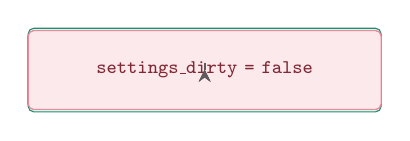
\begin{tikzpicture}[
  b/.style={rounded corners=2pt,draw=ink!50,fill=white,align=center,inner sep=4pt,
            font=\scriptsize\sffamily,text width=42mm,minimum height=10mm},
  k/.style={b,draw=accent!65,fill=accent!12,text=accent!55!black},
  g/.style={b,draw=mint!70!black,fill=mint!18,text=mint!60!black},
]
  \node[b] (a) {a setting changes\\\scriptsize eg. a checkbox in the egui panel};
  \node[k] (b) {\texttt{settings\_dirty = true}};
  \node[b] (c) {\texttt{should\_save()} returns true};
  \node[g] (d) {\textbf{AppKit:} \texttt{refresh()} saves immediately\\\textbf{egui:} \texttt{effects()} waits 2\,s};
  \node[b] (e) {\texttt{save\_settings()}\\\scriptsize \texttt{fs::rename} makes it atomic};
  \node[k] (f) {\texttt{settings\_dirty = false}};
  \draw[e] (a)--(b); \draw[e] (b)--(c); \draw[e] (c)--(d); \draw[e] (d)--(e); \draw[e] (e)--(f);
\end{tikzpicture}
\caption{Saving is deferred, not immediate. The egui shell coalesces writes so that
dragging a slider does not hit the disk on every pixel.}
\label{fig:save}
\end{figure}

\keybox{mint}{%
\textbf{Why \code{fs::rename}?} On all three target platforms \code{rename} within the
same directory is atomic: a reader sees either the old file or the new one, never a
partial write. The \code{.tmp} suffix also means a crashed write leaves a stray file
instead of a truncated \code{settings.conf}.}
\clearpage
\section{Statistics: constant memory by construction}

\file{stats.rs} has a one-line summary in its module doc: \emph{``Streaming CSV storage
and a fixed seven-day cache: memory does not grow with history.''} Everything in the
file exists to make that sentence true.

\subsection{The on-disk format}

\begin{figure}[H]
\centering
\begin{tikzpicture}[x=1mm,y=1mm]
  \draw[draw=softink!30,line width=0.5pt] (0,0) rectangle (150,46);
  % header
  \node[anchor=west,font=\tiny\sffamily\bfseries,text=softink] at (4,40)
    {\texttt{epoch\_seconds, duration\_seconds, activity, completed}};
  % rows
  \foreach \y/\e/\s/\a/\c in {
    32/1759218604/1500/0/1,
    24/17592187544/300/1/1,
    16/17592187844/120/0/0,
    8/17592187964/60/2/0}
  {
    \node[anchor=west,font=\tiny\sffamily] at (4,\y) {\texttt{\e, \s, \a, \c}};
  }
  \node[anchor=west,font=\tiny\sffamily,text=softink] at (4,4)
    {\texttt{activity}: 0 = Session, 1 = ShortBreak, 2 = LongBreak};
  \node[anchor=west,font=\tiny\sffamily,text=softink] at (4,-2)
    {\texttt{completed}: 1 if the activity ran to the end, 0 if it was skipped or stopped};
\end{tikzpicture}
\caption{One line per activity. The file is append-only, so the only write is
\texttt{writeln!} at the end.}
\label{fig:csv}
\end{figure}

\subsection{The scanner: fixed buffers, no allocation}

\begin{figure}[H]
\centering
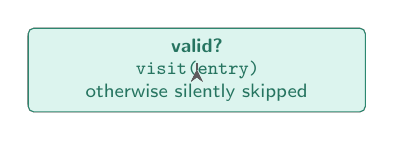
\begin{tikzpicture}[
  b/.style={rounded corners=2pt,draw=ink!50,fill=white,align=center,inner sep=4pt,
            font=\scriptsize\sffamily,text width=40mm,minimum height=10mm},
  k/.style={b,draw=accent!65,fill=accent!12,text=accent!55!black},
  g/.style={b,draw=mint!70!black,fill=mint!18,text=mint!60!black},
]
  \node[b] (a) {\textbf{read 8192 bytes}\\\scriptsize into a stack array};
  \node[b] (b) {\textbf{walk the bytes}\\\scriptsize append to a 256-byte line buffer};
  \node[k] (c) {\textbf{line longer than 255?}\\\texttt{overflow = true}\\\scriptsize the line is dropped, not buffered};
  \node[b] (d) {\textbf{newline?}\\\texttt{Entry::parse(\&line[..len])}};
  \node[g] (e) {\textbf{valid?}\\\texttt{visit(entry)}\\\scriptsize otherwise silently skipped};
  \draw[e] (a)--(b); \draw[e] (b)--(c); \draw[e] (c)--(d); \draw[e] (d)--(e);
\end{tikzpicture}
\caption{\texttt{scan()} uses two fixed stack buffers. A corrupt multi-megabyte line
costs one boolean, not a allocation.}
\label{fig:scan}
\end{figure}

\begin{lstlisting}[caption={\file{stats.rs} lines 190--192. The two buffers are the whole
memory story.}]
let mut chunk = [0; 8192];   // read buffer, on the stack
let mut line  = [0; 256];   // line buffer, on the stack
let (mut len, mut overflow) = (0, false);
\end{lstlisting}

\subsection{The cache: seven days, always}

\begin{figure}[H]
\centering
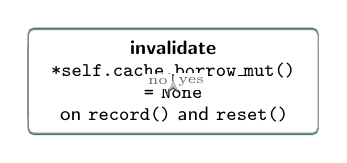
\begin{tikzpicture}[
  c/.style={rounded corners=2pt,draw=ink!50,fill=white,align=center,inner sep=4pt,
            font=\scriptsize\sffamily,text width=34mm,minimum height=10mm},
  h/.style={c,draw=mint!70!black,fill=mint!18,text=mint!60!black},
]
  \node[c] (a) {\textbf{request}\\\texttt{daily\_totals(day, completed\_only)}};
  \node[h] (b) {\textbf{cache hit?}\\\texttt{cache.day == day \&\&\\cache.completed\_only == completed\_only}};
  \node[c] (c) {\textbf{miss: scan the file}\\\scriptsize fold each entry into \texttt{series[(date - day + 6)]}};
  \node[c] (d) {\textbf{store}\\\texttt{Cache \{ day, completed\_only, series \}}};
  \node[c] (e) {\textbf{invalidate}\\\texttt{*self.cache.borrow\_mut() = None}\\\scriptsize on \texttt{record()} and \texttt{reset()}};
  \draw[e] (a)--(b); \draw[e] (b)-- node[vlabel, right, font=\tiny] {yes} (d);
  \draw[e] (b)-- node[vlabel, left, font=\tiny] {no} (c); \draw[e] (c)--(d);
  \draw[ethin, softink!40, dashed] (e) -- (b);
\end{tikzpicture}
\caption{The cache is a \texttt{RefCell<Option<Cache>>}, so \texttt{StatsStore} can stay
\texttt{\&self} in \texttt{record()} and still invalidate itself.}
\label{fig:cache}
\end{figure}

\subsection{What the totals count}

\begin{table}[H]
\centering\small
\begin{tabular}{@{}p{34mm} p{52mm} p{52mm}@{}}
\toprule
\textbf{Field} & \textbf{Incremented when} & \textbf{Notes} \\
\midrule
\texttt{sessions} & a \texttt{Session} entry with \texttt{completed = true} & skipped sessions do not count \\
\texttt{breaks} & a break entry with \texttt{completed = true} & short and long combined \\
\texttt{long\_breaks} & a \texttt{LongBreak} entry with \texttt{completed = true} & a subset of \texttt{breaks} \\
\texttt{skipped} & any entry with \texttt{completed = false} & regardless of activity \\
\texttt{session\_seconds} & every \texttt{Session} entry & completed or not \\
\texttt{break\_seconds} & every break entry & completed or not \\
\bottomrule
\end{tabular}
\caption{\texttt{Totals::add}. The asymmetry is deliberate: seconds are always counted,
but the counters only count completed activities.}
\end{table}

\subsection{Export and reset}

\begin{figure}[H]
\centering
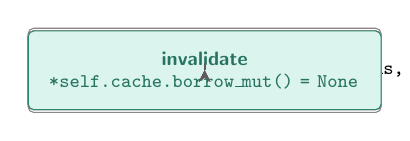
\begin{tikzpicture}[
  b/.style={rounded corners=2pt,draw=ink!50,fill=white,align=center,inner sep=4pt,
            font=\scriptsize\sffamily,text width=42mm,minimum height=10mm},
  k/.style={b,draw=accent!65,fill=accent!12,text=accent!55!black},
  g/.style={b,draw=mint!70!black,fill=mint!18,text=mint!60!black},
]
  \node[b] (a) {\textbf{export\_csv(path)}};
  \node[k] (b) {\textbf{guard}\\\texttt{path == self.path} $\rightarrow$ error\\\scriptsize the log cannot overwrite itself};
  \node[b] (c) {\textbf{write}\\\texttt{date,epoch\_seconds,duration\_seconds,\\activity,completed}};
  \node[g] (d) {\textbf{rename}\\\texttt{.csv.tmp} $\rightarrow$ \texttt{.csv}};
  \node[b] (e) {\textbf{reset()}};
  \node[k] (f) {\textbf{guard}\\\texttt{NotFound} is not an error};
  \node[g] (g) {\textbf{invalidate}\\\texttt{*self.cache.borrow\_mut() = None}};
  \draw[e] (a)--(b); \draw[e] (b)--(c); \draw[e] (c)--(d);
  \draw[e] (e)--(f); \draw[e] (f)--(g);
\end{tikzpicture}
\caption{Both operations are atomic and both invalidate the cache. The export guard is
the only place in the file that returns an error for a reason other than I/O.}
\label{fig:export}
\end{figure}
\clearpage
\section{The AppKit shell}

\file{mac\_shell.rs} is 848 lines and contains no rendering code at all. It builds real
AppKit objects with absolute frames, and lets the operating system draw them.

\subsection{The object graph}

\begin{figure}[H]
\centering
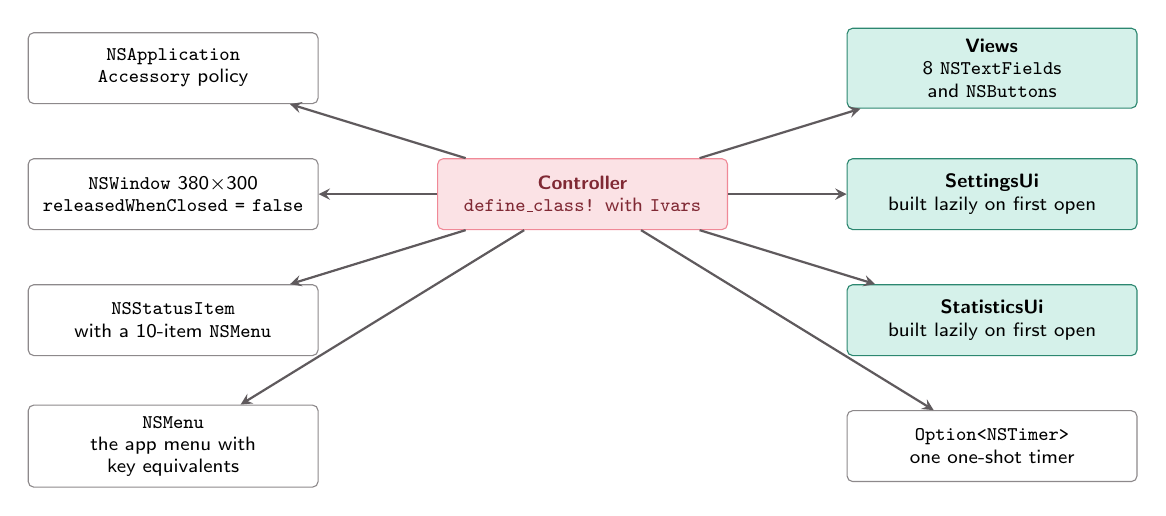
\begin{tikzpicture}[
  o/.style={rounded corners=2pt,draw=ink!50,fill=white,align=center,inner sep=4pt,
            font=\scriptsize\sffamily,text width=34mm,minimum height=9mm},
  c/.style={o,draw=accent!65,fill=intentfill,text=accent!55!black},
  v/.style={o,draw=mint!70!black,fill=shellfill},
]
  \node[c] (ctrl) {\textbf{Controller}\\\scriptsize \texttt{define\_class!} with \texttt{Ivars}};
  \node[o] (app) at (-5.2,1.6) {\texttt{NSApplication}\\\scriptsize \texttt{Accessory} policy};
  \node[o] (win) at (-5.2,0.0) {\texttt{NSWindow} 380$\times$300\\\scriptsize \texttt{releasedWhenClosed = false}};
  \node[o] (bar) at (-5.2,-1.6) {\texttt{NSStatusItem}\\\scriptsize with a 10-item \texttt{NSMenu}};
  \node[o] (menu) at (-5.2,-3.2) {\texttt{NSMenu}\\\scriptsize the app menu with key equivalents};

  \node[v] (views) at (5.2,1.6) {\textbf{Views}\\\scriptsize 8 \texttt{NSTextField}s and \texttt{NSButton}s};
  \node[v] (set) at (5.2,0.0) {\textbf{SettingsUi}\\\scriptsize built lazily on first open};
  \node[v] (stat) at (5.2,-1.6) {\textbf{StatisticsUi}\\\scriptsize built lazily on first open};
  \node[o] (alarm) at (5.2,-3.2) {\texttt{Option<NSTimer>}\\\scriptsize one one-shot timer};

  \draw[e] (ctrl) -- (app); \draw[e] (ctrl) -- (win); \draw[e] (ctrl) -- (bar); \draw[e] (ctrl) -- (menu);
  \draw[e] (ctrl) -- (views); \draw[e] (ctrl) -- (set); \draw[e] (ctrl) -- (stat); \draw[e] (ctrl) -- (alarm);
\end{tikzpicture}
\caption{Every AppKit object is a \texttt{Retained<T>} held in a struct field. Nothing
is leaked, and nothing is freed early: \texttt{objc2} inserts the \texttt{release} calls.}
\label{fig:appkit}
\end{figure}

\subsection{\texttt{refresh()}: the frame callback}

\begin{figure}[H]
\centering
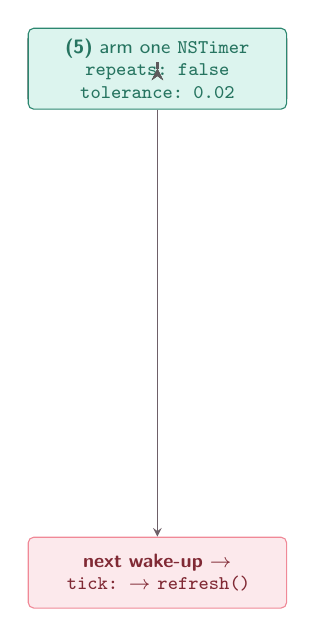
\begin{tikzpicture}[
  s/.style={rounded corners=2pt,draw=ink!50,fill=white,align=center,inner sep=4pt,
            font=\scriptsize\sffamily,text width=30mm,minimum height=9mm},
  k/.style={s,draw=accent!65,fill=accent!12,text=accent!55!black},
  g/.style={s,draw=mint!70!black,fill=mint!18,text=mint!60!black},
]
  \node[s] (r1) {\textbf{(1)} invalidate the old timer\\\scriptsize \texttt{alarm.take()}};
  \node[s] (r2) {\textbf{(2)} update every label\\\scriptsize only if the string changed};
  \node[s] (r3) {\textbf{(3)} consume the flags\\\scriptsize \texttt{mem::take}};
  \node[s] (r4) {\textbf{(4)} save settings\\\scriptsize if \texttt{should\_save()}};
  \node[g] (r5) {\textbf{(5)} arm one \texttt{NSTimer}\\\scriptsize \texttt{repeats: false}\\\texttt{tolerance: 0.02}};
  \foreach \a/\b in {r1/r2,r2/r3,r3/r4,r4/r5} \draw[e] (\a) -- (\b);
  \node[k] (loop) at (0,-6.4) {\textbf{next wake-up} $\rightarrow$ \texttt{tick:} $\rightarrow$ \texttt{refresh()}};
  \draw[ethin, softink] (r5) -- (loop);
\end{tikzpicture}
\caption{\texttt{refresh()} is the only place that touches the views. It is called from
the timer, from every button action, and from the sleep/wake notifications.}
\label{fig:refresh}
\end{figure}

\subsection{The main window layout}

\begin{figure}[H]
\centering
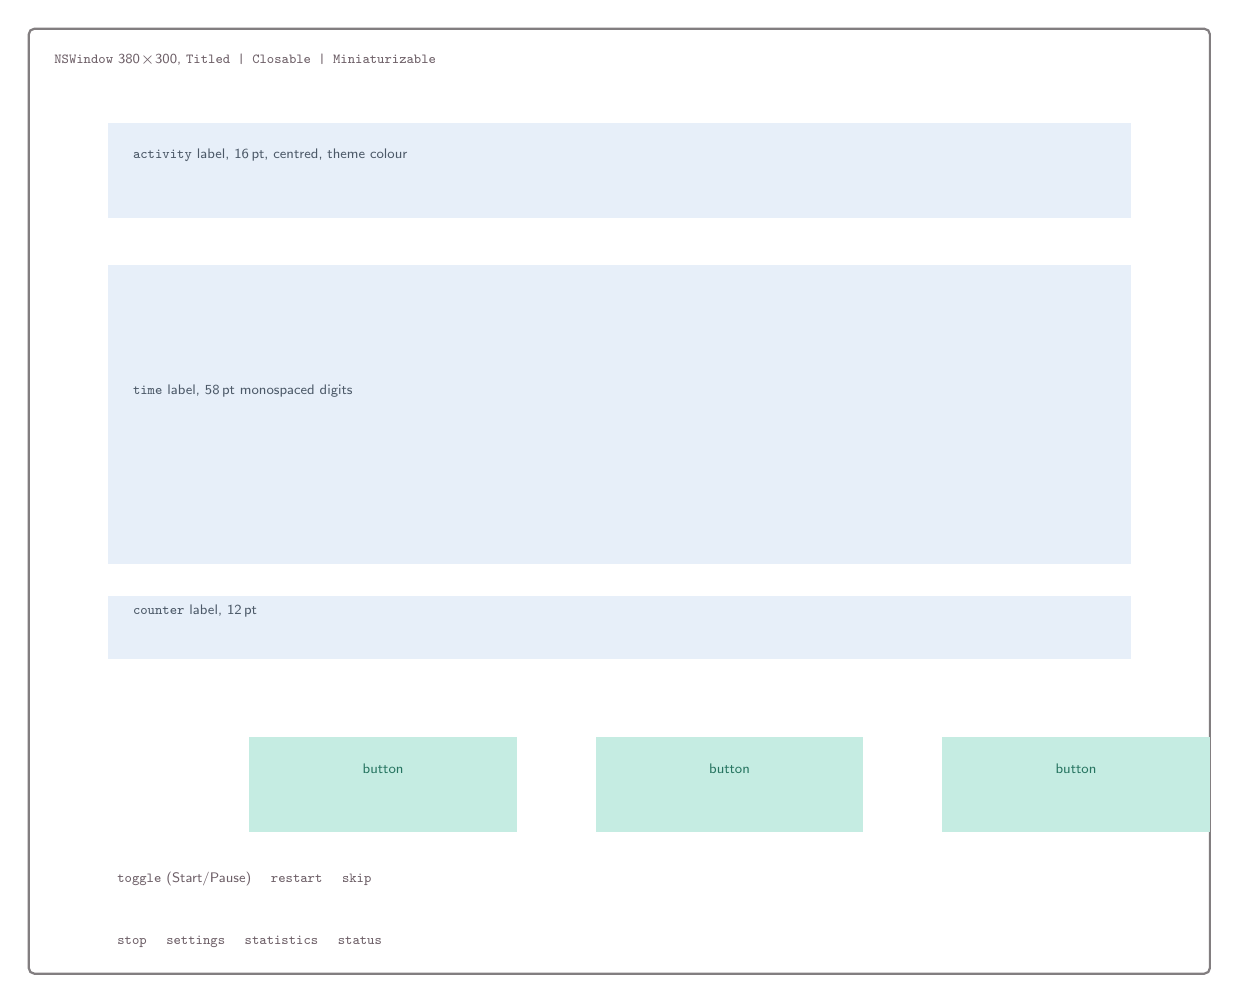
\begin{tikzpicture}[x=1mm,y=1mm]
  \draw[draw=ink!55,line width=0.8pt,rounded corners=2pt] (0,0) rectangle (150,120);
  \node[anchor=west,font=\tiny\sffamily,text=softink] at (2,116) {\texttt{NSWindow} 380$\times$300, \texttt{Titled | Closable | Miniaturizable}};

  \fill[corefill] (10,96) rectangle (140,108);
  \node[anchor=west,font=\tiny\sffamily,text=pastel!45!black] at (12,104) {\texttt{activity} label, 16\,pt, centred, theme colour};

  \fill[corefill] (10,52) rectangle (140,90);
  \node[anchor=west,font=\tiny\sffamily,text=pastel!45!black] at (12,74) {\texttt{time} label, 58\,pt monospaced digits};

  \fill[corefill] (10,40) rectangle (140,48);
  \node[anchor=west,font=\tiny\sffamily,text=pastel!45!black] at (12,46) {\texttt{counter} label, 12\,pt};

  \foreach \x in {28,72,116} {
    \fill[mint!30] (\x,18) rectangle (\x+34,30);
    \node[anchor=center,font=\tiny\sffamily,text=mint!60!black] at ({\x+17},26) {button};
  }
  \node[anchor=west,font=\tiny\sffamily,text=softink] at (10,12)
    {\texttt{toggle} (Start/Pause) \quad \texttt{restart} \quad \texttt{skip}};
  \node[anchor=west,font=\tiny\sffamily,text=softink] at (10,4)
    {\texttt{stop} \quad \texttt{settings} \quad \texttt{statistics} \quad \texttt{status}};
\end{tikzpicture}
\caption{The main window is built with absolute \texttt{NSRect} frames in
\texttt{build()}. There is no auto-layout, so the positions are exact and the window
cannot be resized.}
\label{fig:window}
\end{figure}

\subsection{The action-tag dispatch}

Every button and menu item calls the same \texttt{act:} selector, and the \texttt{tag}
field decides what happens. This is the entire input layer.

\begin{figure}[H]
\centering
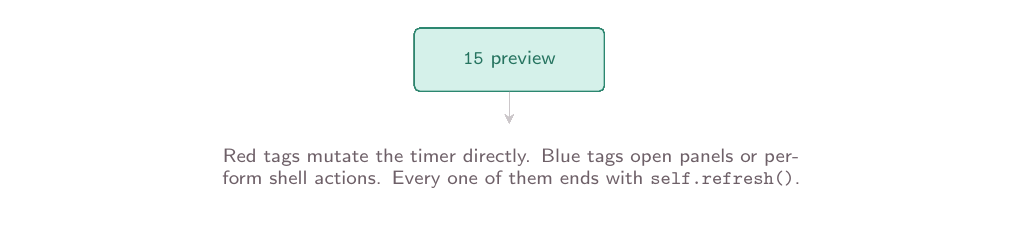
\begin{tikzpicture}[
  t/.style={rounded corners=2pt,draw=ink!50,fill=white,align=center,inner sep=3pt,
            font=\scriptsize\sffamily,text width=22mm,minimum height=8mm},
  a/.style={t,draw=accent!65,fill=accent!12,text=accent!55!black},
  b/.style={t,draw=mint!70!black,fill=shellfill,text=mint!60!black},
]
  \node[a] (t0) {\texttt{0} toggle};
  \node[a] (t1) {\texttt{1} restart};
  \node[a] (t2) {\texttt{2} skip};
  \node[a] (t3) {\texttt{3} stop};
  \node[a] (t4) {\texttt{4} finish};
  \node[b] (t5) {\texttt{5} show};
  \node[b] (t6) {\texttt{6} settings};
  \node[b] (t7) {\texttt{7} statistics};
  \node[b] (t8) {\texttt{8} reset counter};
  \node[b] (t9) {\texttt{9} quit};
  \node[b] (t10) {\texttt{10} apply};
  \node[b] (t11) {\texttt{11} export};
  \node[b] (t12) {\texttt{12} reset stats};
  \node[b] (t13) {\texttt{13} today};
  \node[b] (t14) {\texttt{14} week};
  \node[b] (t15) {\texttt{15} preview};

  \foreach \n in {t0,t1,t2,t3,t4,t5,t6,t7,t8,t9,t10,t11,t12,t13,t14,t15} {
    \draw[ethin, softink!35] (\n.south) -- ++(0,-4mm);
  }
  \node[note, below=6mm of t7, text width=120mm] {%
    Red tags mutate the timer directly. Blue tags open panels or perform shell actions.
    Every one of them ends with \texttt{self.refresh()}.};
\end{tikzpicture}
\caption{Sixteen tags, one selector. Adding a control means adding a \texttt{tag} and a
line in the \texttt{match}.}
\label{fig:tags}
\end{figure}

\subsection{Window closing is not quitting}

\begin{figure}[H]
\centering
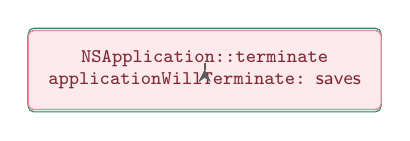
\begin{tikzpicture}[
  b/.style={rounded corners=2pt,draw=ink!50,fill=white,align=center,inner sep=4pt,
            font=\scriptsize\sffamily,text width=42mm,minimum height=10mm},
  k/.style={b,draw=accent!65,fill=accent!12,text=accent!55!black},
  g/.style={b,draw=mint!70!black,fill=mint!18,text=mint!60!black},
]
  \node[b] (a) {user closes the\\\texttt{main window}};
  \node[k] (b) {\texttt{windowShouldClose:}\\\scriptsize returns \texttt{false}};
  \node[g] (c) {\texttt{window.orderOut(None)}\\\scriptsize the window hides, the app keeps running};
  \node[b] (d) {user closes a\\\texttt{panel window}};
  \node[g] (e) {\texttt{apply\_controls()}\\\scriptsize settings are saved on close};
  \node[b] (f) {user picks\\\texttt{Quit}};
  \node[k] (g) {\texttt{NSApplication::terminate}\\\scriptsize \texttt{applicationWillTerminate:} saves};
  \draw[e] (a)--(b); \draw[e] (b)--(c);
  \draw[e] (d)--(e);
  \draw[e] (f)--(g);
\end{tikzpicture}
\caption{\texttt{applicationShouldTerminateAfterLastWindowClosed} returns \texttt{false},
so closing the window never quits the app. The menu bar item is the way back.}
\label{fig:close}
\end{figure}
\clearpage
\section{The egui shell}

\file{egui\_shell.rs} is 170 lines and contains no timer logic. It is a translation
layer: it turns egui events into \texttt{App} method calls, and it turns \texttt{App}'s
intent flags into egui commands.

\subsection{The two callbacks}

egui's \texttt{App} trait has two methods, and the split between them is the whole
design.

\begin{figure}[H]
\centering
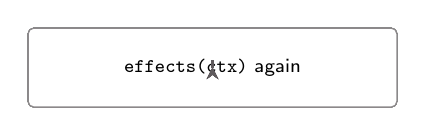
\begin{tikzpicture}[
  b/.style={rounded corners=2pt,draw=ink!50,fill=white,align=center,inner sep=4pt,
            font=\scriptsize\sffamily,text width=44mm,minimum height=10mm},
  k/.style={b,draw=accent!65,fill=accent!12,text=accent!55!black},
  g/.style={b,draw=mint!70!black,fill=mint!18,text=mint!60!black},
]
  \node[k] (l) {\textbf{logic()}\\\scriptsize called when egui needs input};
  \node[b] (l1) {drain the \texttt{Command} queue};
  \node[b] (l2) {handle the window-close request};
  \node[b] (l3) {\texttt{app.tick()}};
  \node[b] (l4) {\texttt{effects(ctx)}};
  \node[g] (u) {\textbf{ui()}\\\scriptsize called to produce the frame};
  \node[b] (u1) {\texttt{app.handle\_keys(ctx)}};
  \node[b] (u2) {\texttt{ui::main::draw}};
  \node[b] (u3) {\texttt{ui::settings::draw}};
  \node[b] (u4) {\texttt{ui::statistics::draw}};
  \node[b] (u5) {\texttt{effects(ctx)} again};
  \draw[e] (l)--(l1); \draw[e] (l1)--(l2); \draw[e] (l2)--(l3); \draw[e] (l3)--(l4);
  \draw[e] (u)--(u1); \draw[e] (u1)--(u2); \draw[e] (u2)--(u3); \draw[e] (u3)--(u4); \draw[e] (u4)--(u5);
\end{tikzpicture}
\caption{\texttt{logic()} mutates, \texttt{ui()} draws. \texttt{effects()} runs in both,
so a flag raised while drawing is still handled in the same frame.}
\label{fig:logicui}
\end{figure}

\subsection{\texttt{effects()}: the egui equivalent of \texttt{refresh()}}

\begin{figure}[H]
\centering
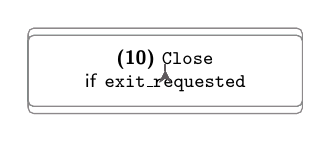
\begin{tikzpicture}[
  s/.style={rounded corners=2pt,draw=ink!50,fill=white,align=center,inner sep=4pt,
            font=\scriptsize\sffamily,text width=32mm,minimum height=9mm},
  k/.style={s,draw=accent!65,fill=accent!12,text=accent!55!black},
  g/.style={s,draw=mint!70!black,fill=mint!18,text=mint!60!black},
]
  \node[s] (e1) {\textbf{(1)} apply the theme\\\scriptsize if \texttt{applied\_theme} changed};
  \node[s] (e2) {\textbf{(2)} apply \texttt{keep\_in\_front}\\\scriptsize \texttt{WindowLevel}};
  \node[s] (e3) {\textbf{(3)} consume \texttt{hide\_requested}\\\scriptsize \texttt{Visible(false)}};
  \node[s] (e4) {\textbf{(4)} consume \texttt{show\_requested}\\\scriptsize \texttt{Focus}};
  \node[s] (e5) {\textbf{(5)} consume \texttt{notify\_requested}\\\scriptsize \texttt{native::play}};
  \node[s] (e6) {\textbf{(6)} consume \texttt{tick\_requested}\\\scriptsize \texttt{play(Tink)}};
  \node[s] (e7) {\textbf{(7)} update the menu bar\\\scriptsize \texttt{native.update}};
  \node[g] (e8) {\textbf{(8)} schedule the repaint\\\scriptsize \texttt{schedule\_repaint}};
  \node[s] (e9) {\textbf{(9)} save settings\\\scriptsize after a 2\,s debounce};
  \node[s] (e10) {\textbf{(10)} \texttt{Close}\\\scriptsize if \texttt{exit\_requested}};
  \foreach \i/\j in {e1/e2,e2/e3,e3/e4,e4/e5,e5/e6,e6/e7,e7/e8,e8/e9,e9/e10}
    \draw[e] (\i) -- (\j);
\end{tikzpicture}
\caption{Ten steps, in order. Steps 1--2 are idempotent state syncs, 3--6 are the intent
flags, and 7--10 are the shell's own bookkeeping.}
\label{fig:effects}
\end{figure}

\subsection{The \texttt{Command} queue}

\file{native.rs} turns AppKit events into an enum and queues them. The shell drains the
queue once per frame.

\begin{figure}[H]
\centering
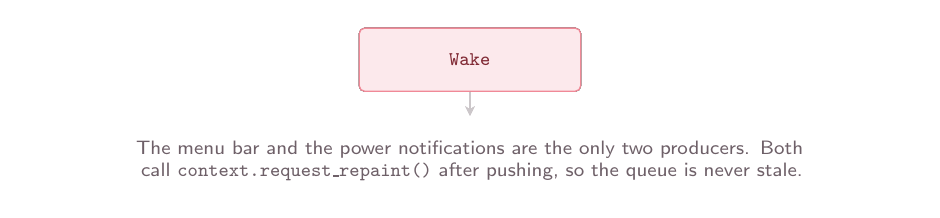
\begin{tikzpicture}[
  c/.style={rounded corners=2pt,draw=ink!50,fill=white,align=center,inner sep=3pt,
            font=\scriptsize\sffamily,text width=26mm,minimum height=8mm},
  q/.style={c,draw=accent!65,fill=accent!12,text=accent!55!black},
]
  \node[c] (m0) {\texttt{0} Toggle};
  \node[c] (m1) {\texttt{1} Restart};
  \node[c] (m2) {\texttt{2} Skip};
  \node[c] (m3) {\texttt{3} Stop};
  \node[c] (m4) {\texttt{4} Finish};
  \node[c] (m5) {\texttt{5} Show};
  \node[c] (m6) {\texttt{6} Settings};
  \node[c] (m7) {\texttt{7} Statistics};
  \node[c] (m8) {\texttt{8} ResetCounter};
  \node[c] (m9) {\texttt{9} Quit};
  \node[q] (s1) {\texttt{Sleep}};
  \node[q] (s2) {\texttt{Wake}};
  \foreach \n in {m0,m1,m2,m3,m4,m5,m6,m7,m8,m9,s1,s2}
    \draw[ethin, softink!35] (\n.south) -- ++(0,-3mm);
  \node[note, below=5mm of m4, text width=110mm] {%
    The menu bar and the power notifications are the only two producers. Both call
    \texttt{context.request\_repaint()} after pushing, so the queue is never stale.};
\end{tikzpicture}
\caption{Twelve \texttt{Command} variants. The \texttt{tag} on each \texttt{NSMenuItem}
is the discriminant, so adding a menu item is a one-line change in \file{native.rs} and
one \texttt{match} arm in \file{egui\_shell.rs}.}
\label{fig:command}
\end{figure}

\subsection{Closing the window hides it}

\begin{figure}[H]
\centering
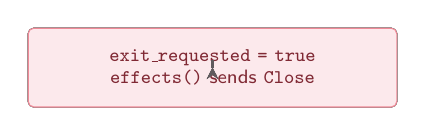
\begin{tikzpicture}[
  b/.style={rounded corners=2pt,draw=ink!50,fill=white,align=center,inner sep=4pt,
            font=\scriptsize\sffamily,text width=44mm,minimum height=10mm},
  k/.style={b,draw=accent!65,fill=accent!12,text=accent!55!black},
  g/.style={b,draw=mint!70!black,fill=mint!18,text=mint!60!black},
]
  \node[b] (a) {user clicks the\\\texttt{close button}};
  \node[k] (b) {\texttt{close\_requested()}\\\scriptsize and \texttt{exit\_requested} is false};
  \node[g] (c) {\texttt{CancelClose}\\\scriptsize the window stays alive};
  \node[g] (d) {\texttt{hide\_requested = true}\\\scriptsize \texttt{effects()} hides it};
  \node[b] (e) {user picks\\\texttt{Quit}};
  \node[k] (f) {\texttt{exit\_requested = true}\\\scriptsize \texttt{effects()} sends \texttt{Close}};
  \draw[e] (a)--(b); \draw[e] (b)--(c); \draw[e] (c)--(d);
  \draw[e] (e)--(f);
\end{tikzpicture}
\caption{The egui shell reproduces the AppKit shell's behaviour: closing hides, quitting
terminates. The \texttt{CancelClose} command is what makes the first part work.}
\label{fig:egui-close}
\end{figure}

\subsection{The dial}

\begin{figure}[H]
\centering
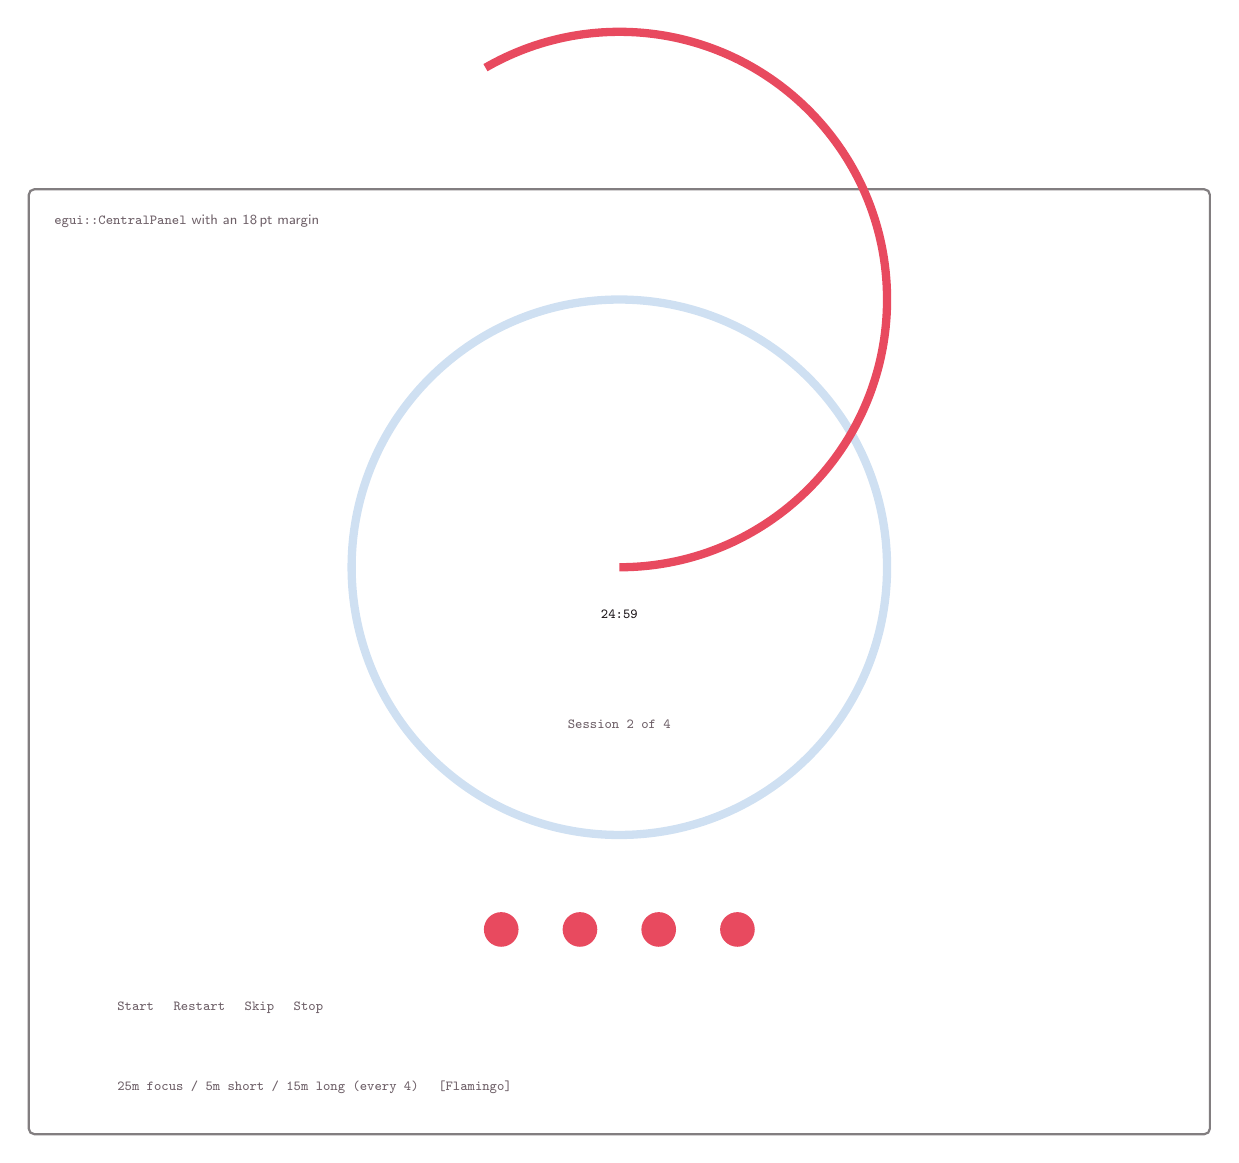
\begin{tikzpicture}[x=1mm,y=1mm]
  \draw[draw=ink!55,line width=0.8pt,rounded corners=2pt] (0,0) rectangle (150,120);
  \node[anchor=west,font=\tiny\sffamily,text=softink] at (2,116)
    {\texttt{egui::CentralPanel} with an 18\,pt margin};

  \draw[pastel!55, line width=3] (75,72) circle (34);
  \draw[accent, line width=3] (75,72) arc[start angle=-90,end angle=120,radius=34];
  \node[anchor=center,font=\tiny\sffamily,text=ink] at (75,66) {\texttt{24:59}};
  \node[anchor=center,font=\tiny\sffamily,text=softink] at (75,52) {\texttt{Session 2 of 4}};

  \foreach \i in {0,1,2,3} {
    \fill[accent] ({60+\i*10},26) circle (2.2);
  }
  \node[anchor=west,font=\tiny\sffamily,text=softink] at (10,16)
    {\texttt{Start} \quad \texttt{Restart} \quad \texttt{Skip} \quad \texttt{Stop}};
  \node[anchor=west,font=\tiny\sffamily,text=softink] at (10,6)
    {\texttt{25m focus / 5m short / 15m long (every 4)} \quad \texttt{[Flamingo]}};
\end{tikzpicture}
\caption{The main panel is drawn with \texttt{painter} calls, not widgets. The progress
arc is a polyline of 96 points, which avoids both polygon triangulation and an image
texture.}
\label{fig:dial}
\end{figure}
\clearpage
\section{Input: three paths to the same methods}

There are exactly three ways to reach the timer: keyboard, menu bar, and buttons. All
three end at the same \texttt{App} methods.

\subsection{Keyboard}

\begin{figure}[H]
\centering
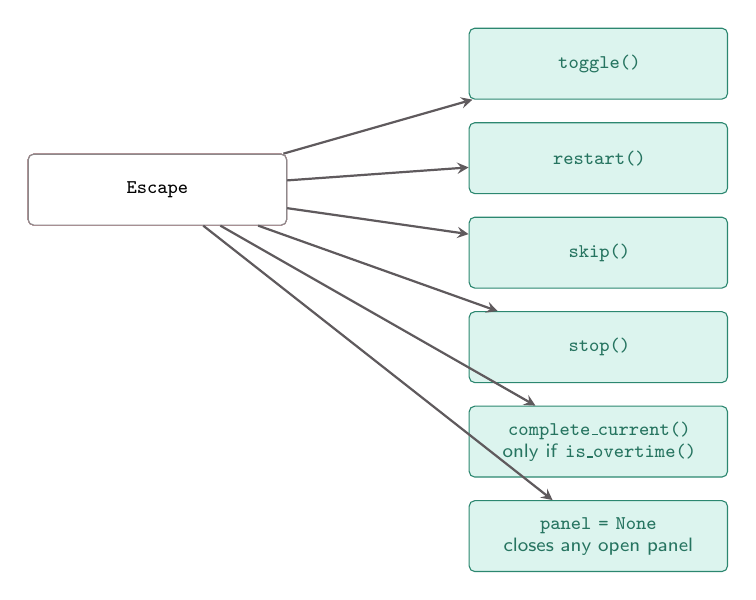
\begin{tikzpicture}[
  k/.style={rounded corners=2pt,draw=ink!50,fill=white,align=center,inner sep=4pt,
            font=\scriptsize\sffamily,text width=30mm,minimum height=9mm},
  g/.style={k,draw=mint!70!black,fill=mint!18,text=mint!60!black},
  a/.style={k,draw=accent!65,fill=accent!12,text=accent!55!black},
]
  \node[k] (sp) {\texttt{Space}};
  \node[k] (r) {\texttt{R}};
  \node[k] (s) {\texttt{S}};
  \node[k] (x) {\texttt{X}};
  \node[a] (f) {\texttt{F}};
  \node[k] (esc) {\texttt{Escape}};

  \node[g] (t1) at (5.6,1.6) {\texttt{toggle()}};
  \node[g] (t2) at (5.6,0.4) {\texttt{restart()}};
  \node[g] (t3) at (5.6,-0.8) {\texttt{skip()}};
  \node[g] (t4) at (5.6,-2.0) {\texttt{stop()}};
  \node[g] (t5) at (5.6,-3.2) {\texttt{complete\_current()}\\\scriptsize only if \texttt{is\_overtime()}};
  \node[g] (t6) at (5.6,-4.4) {\texttt{panel = None}\\\scriptsize closes any open panel};

  \draw[e] (sp)--(t1); \draw[e] (r)--(t2); \draw[e] (s)--(t3);
  \draw[e] (x)--(t4); \draw[e] (f)--(t5); \draw[e] (esc)--(t6);
\end{tikzpicture}
\caption{Six keys. \texttt{Escape} is handled first and closes the panel; the other five
are ignored while a panel is open or while egui wants the keyboard.}
\label{fig:keys}
\end{figure}

\begin{lstlisting}[caption={\file{app.rs} lines 190--216. The guard at the top is what
keeps the timer from reacting while the user is typing in a settings field.}]
pub fn handle_keys(&mut self, ctx: &egui::Context) {
    let escape = ctx.input(|i| i.key_pressed(egui::Key::Escape));
    if escape { self.panel = Panel::None; self.confirm_reset = false; }
    if ctx.egui_wants_keyboard_input() || self.panel != Panel::None { return; }
    ctx.input(|i| {
        if i.key_pressed(egui::Key::Space) { self.toggle(); }
        if i.key_pressed(egui::Key::R)     { self.restart(); }
        if i.key_pressed(egui::Key::S)     { self.skip(); }
        if i.key_pressed(egui::Key::X)     { self.stop(); }
        if i.key_pressed(egui::Key::F) && self.is_overtime() { self.complete_current(); }
    });
}
\end{lstlisting}

\subsection{Global hotkeys, without a keyboard tap}

The AppKit shell registers five Carbon hotkeys. They work even when the app is not
focused, and they need no permission prompt because they are registered on the
application's own event target.

\begin{figure}[H]
\centering
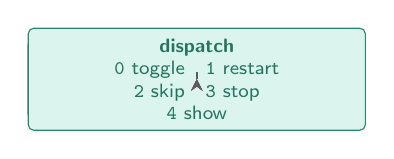
\begin{tikzpicture}[
  b/.style={rounded corners=2pt,draw=ink!50,fill=white,align=center,inner sep=4pt,
            font=\scriptsize\sffamily,text width=40mm,minimum height=10mm},
  k/.style={b,draw=accent!65,fill=accent!12,text=accent!55!black},
  g/.style={b,draw=mint!70!black,fill=mint!18,text=mint!60!black},
]
  \node[b] (a) {\textbf{RegisterEventHotKey}\\\scriptsize Control + Option};
  \node[b] (b) {\textbf{key codes}\\\texttt{49} Space\quad \texttt{15} R\quad \texttt{1} S\\\texttt{7} X\quad \texttt{17} T};
  \node[b] (c) {\textbf{InstallEventHandler}\\\scriptsize on \texttt{GetApplicationEventTarget()}};
  \node[k] (d) {\textbf{callback}\\\texttt{key\_id(event)}\\\scriptsize checks the \texttt{TMRs} signature};
  \node[g] (e) {\textbf{dispatch}\\\texttt{0} toggle\quad \texttt{1} restart\\\texttt{2} skip\quad \texttt{3} stop\\\texttt{4} show};
  \draw[e] (a)--(b); \draw[e] (b)--(c); \draw[e] (c)--(d); \draw[e] (d)--(e);
\end{tikzpicture}
\caption{\file{hotkeys.rs} is 128 lines of raw Carbon FFI. The \texttt{TMRs} signature
is a magic value that stops the handler from reacting to some other app's hotkey.}
\label{fig:hotkeys}
\end{figure}

\begin{table}[H]
\centering\small
\begin{tabular}{@{}p{22mm} p{26mm} p{30mm} p{60mm}@{}}
\toprule
\textbf{Key code} & \textbf{Key} & \textbf{Modifiers} & \textbf{Action} \\
\midrule
49 & Space & Control + Option & \texttt{toggle()} \\
15 & R & Control + Option & \texttt{restart()} \\
1 & S & Control + Option & \texttt{skip()} \\
7 & X & Control + Option & \texttt{stop()} \\
17 & T & Control + Option & \texttt{show()} \\
\bottomrule
\end{tabular}
\caption{The five registered hotkeys. The \texttt{T} key is the ``show timer'' command;
it is the only one that does not mutate the timer.}
\end{table}

\subsection{The menu bar}

\begin{figure}[H]
\centering
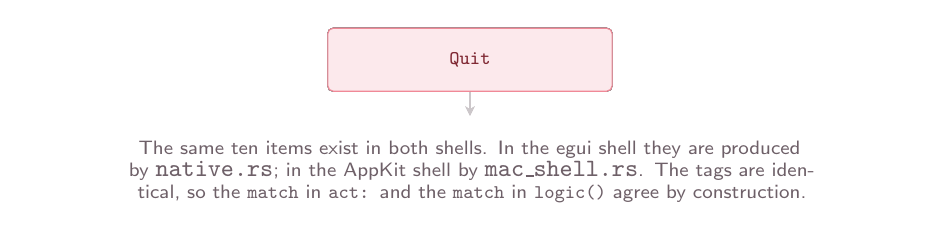
\begin{tikzpicture}[
  m/.style={rounded corners=2pt,draw=ink!50,fill=white,align=center,inner sep=3pt,
            font=\scriptsize\sffamily,text width=34mm,minimum height=8mm},
  h/.style={m,draw=accent!65,fill=accent!12,text=accent!55!black},
]
  \node[m] (i0) {\texttt{Start / Pause}};
  \node[m] (i1) {\texttt{Restart}};
  \node[m] (i2) {\texttt{Skip}};
  \node[m] (i3) {\texttt{Stop}};
  \node[m] (i4) {\texttt{Finish overtime}};
  \node[m] (i5) {\texttt{Show timer}};
  \node[m] (i6) {\texttt{Settings...}};
  \node[m] (i7) {\texttt{Statistics...}};
  \node[m] (i8) {\texttt{Reset session counter}};
  \node[h] (i9) {\texttt{Quit}};
  \foreach \n in {i0,i1,i2,i3,i4,i5,i6,i7,i8,i9}
    \draw[ethin, softink!35] (\n.south) -- ++(0,-3mm);
  \node[note, below=5mm of i4, text width=110mm] {%
    The same ten items exist in both shells. In the egui shell they are produced by
    \file{native.rs}; in the AppKit shell by \file{mac\_shell.rs}. The tags are identical,
    so the \texttt{match} in \texttt{act:} and the \texttt{match} in \texttt{logic()}
    agree by construction.};
\end{tikzpicture}
\caption{Ten menu items. The first item's title tracks the run state, so the menu bar
always says \texttt{Start}, \texttt{Pause}, or \texttt{Resume}.}
\label{fig:menubar}
\end{figure}
\clearpage
\section{Themes}

Five themes, each a \texttt{Palette} of five colours. The AppKit shell uses one of them
for a single label; the egui shell pushes all five into the global style.

\subsection{The five palettes}

\begin{figure}[H]
\centering
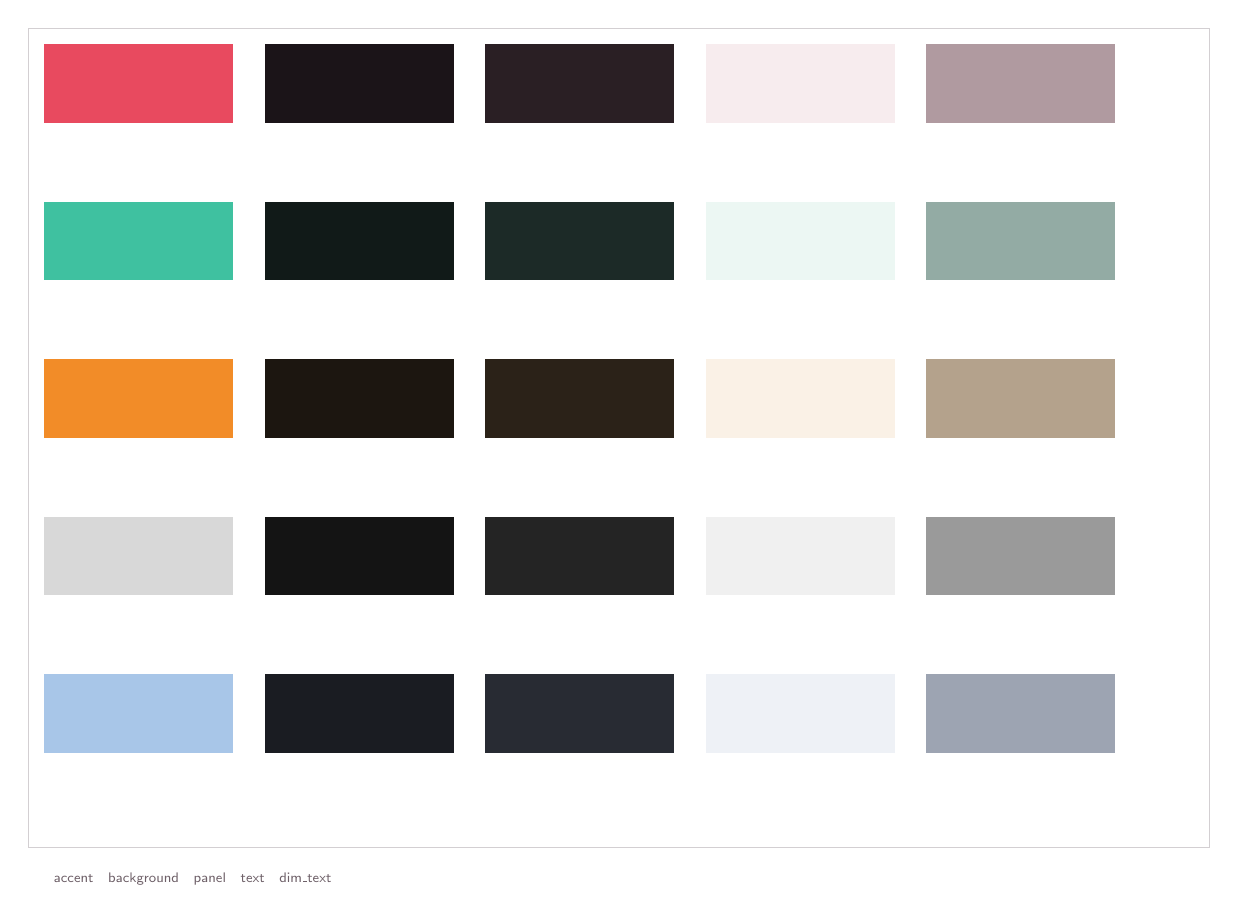
\begin{tikzpicture}[x=1mm,y=1mm]
  \draw[draw=softink!30,line width=0.5pt] (0,0) rectangle (150,104);

  % one row per theme: name + five swatches
  \foreach \i/\name/\ca/\cb/\cp/\ct/\cd in {
    0/Flamingo/t0a/t0b/t0p/t0t/t0d,
    1/Mint/t1a/t1b/t1p/t1t/t1d,
    2/Mandarin/t2a/t2b/t2p/t2t/t2d,
    3/Monochrome/t3a/t3b/t3p/t3t/t3d,
    4/Pastel/t4a/t4b/t4p/t4t/t4d}
  {
    \pgfmathsetmacro{\y}{92-\i*20}
    \node[anchor=west,font=\tiny\sffamily\bfseries,text=ink] at (2,{\y+8}) {\name};
    \fill[\ca]  (2,{\y})       rectangle (26,{\y+10});
    \fill[\cb]  (30,{\y})      rectangle (54,{\y+10});
    \fill[\cp]  (58,{\y})      rectangle (82,{\y+10});
    \fill[\ct]  (86,{\y})      rectangle (110,{\y+10});
    \fill[\cd]  (114,{\y})     rectangle (138,{\y+10});
  }
  \node[anchor=west,font=\tiny\sffamily,text=softink] at (2,-4)
    {accent\quad background\quad panel\quad text\quad dim\_text};
\end{tikzpicture}
\caption{The five palettes from \file{theme.rs}. Every one of them is dark, and every
accent is bright enough to read against its own background.}
\label{fig:themes}
\end{figure}

\subsection{How a theme reaches the screen}

\begin{figure}[H]
\centering
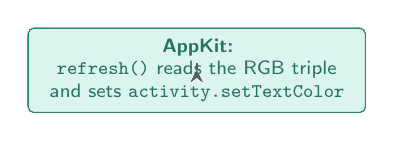
\begin{tikzpicture}[
  b/.style={rounded corners=2pt,draw=ink!50,fill=white,align=center,inner sep=4pt,
            font=\scriptsize\sffamily,text width=40mm,minimum height=10mm},
  k/.style={b,draw=accent!65,fill=accent!12,text=accent!55!black},
  g/.style={b,draw=mint!70!black,fill=mint!18,text=mint!60!black},
]
  \node[b] (a) {\textbf{user picks a theme}\\\scriptsize combo box in the footer or settings};
  \node[k] (b) {\texttt{app.set\_theme(theme)}};
  \node[b] (c) {\texttt{settings.theme = theme}\\\texttt{apply\_settings()}\\\texttt{palette = palette(theme)}};
  \node[g] (d) {\textbf{egui:}\\\texttt{theme::apply(ctx, palette)}\\\scriptsize rewrites \texttt{visuals} and \texttt{text\_styles}};
  \node[g] (e) {\textbf{AppKit:}\\\texttt{refresh()} reads the RGB triple\\\scriptsize and sets \texttt{activity.setTextColor}};
  \draw[e] (a)--(b); \draw[e] (b)--(c); \draw[e] (c)--(d); \draw[e] (c)--(e);
\end{tikzpicture}
\caption{One \texttt{Palette} struct, two very different applications of it. The egui
path rewrites the global style; the AppKit path sets one colour on one label.}
\label{fig:themepath}
\end{figure}

\subsection{The font}

\begin{figure}[H]
\centering
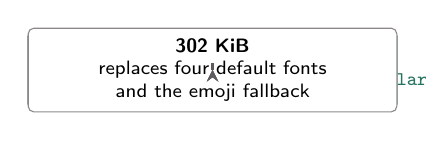
\begin{tikzpicture}[
  b/.style={rounded corners=2pt,draw=ink!50,fill=white,align=center,inner sep=4pt,
            font=\scriptsize\sffamily,text width=44mm,minimum height=10mm},
  g/.style={b,draw=mint!70!black,fill=mint!18,text=mint!60!black},
]
  \node[b] (a) {\textbf{one font file}\\\texttt{assets/Hack-Regular.ttf}};
  \node[g] (b) {\textbf{embedded at compile time}\\\texttt{include\_bytes!("../assets/Hack-Regular.ttf")}};
  \node[b] (c) {\textbf{installed for both families}\\\texttt{Proportional} and \texttt{Monospace}};
  \node[b] (d) {\textbf{302 KiB}\\\scriptsize replaces four default fonts and the emoji fallback};
  \draw[e] (a)--(b); \draw[e] (b)--(c); \draw[e] (c)--(d);
\end{tikzpicture}
\caption{The font is the only binary asset in the project. There are no icons, no images,
and no sound files.}
\label{fig:font}
\end{figure}
\clearpage
\section{The release build}

\subsection{The profile}

\begin{figure}[H]
\centering
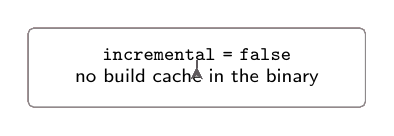
\begin{tikzpicture}[
  b/.style={rounded corners=2pt,draw=ink!50,fill=white,align=center,inner sep=4pt,
            font=\scriptsize\sffamily,text width=40mm,minimum height=10mm},
  k/.style={b,draw=accent!65,fill=accent!12,text=accent!55!black},
  g/.style={b,draw=mint!70!black,fill=mint!18,text=mint!60!black},
]
  \node[b] (a) {\texttt{opt-level = "z"}\\\scriptsize optimise for size, not speed};
  \node[b] (b) {\texttt{lto = true}\\\scriptsize fat LTO across the whole crate};
  \node[b] (c) {\texttt{codegen-units = 1}\\\scriptsize one unit, so LTO sees everything};
  \node[k] (d) {\texttt{panic = "abort"}\\\scriptsize no unwinding machinery};
  \node[b] (e) {\texttt{strip = true}\\\scriptsize no symbol table};
  \node[b] (f) {\texttt{incremental = false}\\\scriptsize no build cache in the binary};
  \draw[e] (a)--(b); \draw[e] (b)--(c); \draw[e] (c)--(d); \draw[e] (d)--(e); \draw[e] (e)--(f);
\end{tikzpicture}
\caption{Six settings, all aimed at the same goal. The README is explicit that these
should be measured, not trusted: \texttt{ls -lh target/release/tomito} and an idle
memory reading are the real evidence.}
\label{fig:profile}
\end{figure}

\subsection{Packaging}

\begin{figure}[H]
\centering
\begin{tikzpicture}[
  b/.style={rounded corners=2pt,draw=ink!50,fill=white,align=center,inner sep=4pt,
            font=\scriptsize\sffamily,text width=40mm,minimum height=10mm},
  g/.style={b,draw=mint!70!black,fill=mint!18,text=mint!60!black},
]
  \node[b] (a) {\texttt{cargo build --locked --release}};
  \node[b] (b) {\texttt{cp target/release/tomito}\\\texttt{dist/Tomito RS.app/Contents/MacOS/}};
  \node[b] (c) {\texttt{cp packaging/Info.plist}\\\texttt{Contents/Info.plist}};
  \node[g] (d) {\texttt{codesign --force --sign -}\\\scriptsize ad-hoc signature};
  \node[b] (e) {\texttt{du -sh "dist/Tomito RS.app"}};
  \draw[e] (a)--(b); \draw[e] (b)--(c); \draw[e] (c)--(d); \draw[e] (d)--(e);
\end{tikzpicture}
\caption{\file{scripts/package-macos.sh} is five commands. There is no DMG, no notarisation,
and no installer.}
\label{fig:package}
\end{figure}

\subsection{What is deliberately not implemented}

\begin{table}[H]
\centering\small
\begin{tabular}{@{}p{44mm} p{96mm}@{}}
\toprule
\textbf{Feature} & \textbf{Why it is absent} \\
\midrule
Menu-bar status item (egui build) & \file{native.rs} provides one, but the egui build does not use it \\
AppleScript command suite & needs a scripting dictionary and \texttt{sdef} tooling \\
Global hotkeys (egui build) & Carbon only; the egui build has app-focused keys only \\
Sleep and wake handling (egui build) & \file{native.rs} provides it, but only on macOS \\
Audio playback & sound names are stored and \texttt{NSSound::soundNamed} is called, but no audio files are bundled \\
Wayland & the \texttt{eframe} features are \texttt{glow} and \texttt{x11} only \\
\bottomrule
\end{tabular}
\caption{The README's ``Not implemented'' list. Each item is a platform API that lies
outside the egui scope of this build, not a missing piece of the core.}
\end{table}

\subsection{The size and memory posture}

\begin{figure}[H]
\centering
\begin{tikzpicture}[
  b/.style={rounded corners=2pt,draw=ink!50,fill=white,align=center,inner sep=4pt,
            font=\scriptsize\sffamily,text width=42mm,minimum height=10mm},
  g/.style={b,draw=mint!70!black,fill=mint!18,text=mint!60!black},
]
  \node[b] (a) {\textbf{renderer}\\\texttt{glow}, not \texttt{wgpu}};
  \node[b] (b) {\textbf{eframe defaults}\\\texttt{default-features = false}};
  \node[b] (c) {\textbf{no textures}\\\scriptsize the dial is a polyline, not an image};
  \node[b] (d) {\textbf{no icon fonts}\\\scriptsize one TTF, no emoji fallback};
  \node[b] (e) {\textbf{no threads}\\\scriptsize no async runtime, no background work};
  \node[g] (f) {\textbf{repaint budget}\\\scriptsize one wake-up per displayed second};
  \draw[e] (a)--(b); \draw[e] (b)--(c); \draw[e] (c)--(d); \draw[e] (d)--(e); \draw[e] (e)--(f);
\end{tikzpicture}
\caption{Seven independent decisions that each shave something off the binary. None of
them is a compromise in behaviour: the timer still works identically.}
\label{fig:posture}
\end{figure}
\clearpage
\section{What the tests actually prove}

There are 31 tests. They are all in \texttt{\#[cfg(test)]} modules inside the files they
test, which means they compile with the same \texttt{cfg} gates as the code.

\subsection{The test map}

\noindent\textbf{\textcolor{pastel!45!black}{\texttt{timer.rs}}}\\[0.4em]
\hspace{1.4em}14 tests\par
\begin{itemize}[leftmargin=1.4em,itemsep=0.15em,topsep=0.1em]
\item \texttt{starts\_idle\_\allowbreak on\_a\_session} --- initial state is Idle/Session with the full duration
\item \texttt{session\_cycles\_\allowbreak into\_short\_then\_long\_breaks} --- the 4th finished session earns a LongBreak
\item \texttt{skip\_moves\_\allowbreak on\_without\_counting\_a\_session} --- skipping does not increment the counter
\item \texttt{disable\_breaks\_\allowbreak jumps\_straight\_back\_to\_a\_session} --- the setting is honoured in \texttt{advance()}
\item \texttt{disable\_long\_breaks\_\allowbreak keeps\_only\_short\_breaks} --- the cycle counter still runs
\item \texttt{pause\_stops\_\allowbreak elapsed\_time} --- elapsed is frozen across a pause
\item \texttt{stop\_resets\_\allowbreak the\_current\_activity} --- elapsed goes to zero, activity is kept
\item \texttt{restart\_clears\_\allowbreak progress\_but\_keeps\_running} --- the run state survives a restart
\item \texttt{progress\_and\_\allowbreak remaining\_track\_the\_activity} --- both are derived from elapsed
\item \texttt{remaining\_display\_\allowbreak rounds\_up\_whole\_seconds} --- a fresh timer shows 25:00, not 24:59
\item \texttt{exact\_and\_\allowbreak fractional\_rounding\_and\_deadlines} --- \texttt{next\_display\_change()} returns the complement
\item \texttt{skipped\_session\_at\_cycle\_boundary\_\allowbreak does\_not\_\allowbreak schedule\_long\_break} --- the \texttt{completion == Finished} check
\item \texttt{running\_duration\_change\_\allowbreak clamps\_actual\_progress} --- \texttt{saturating\_sub} prevents underflow
\item \texttt{new\_settings\_\allowbreak reshape\_the\_current\_activity} --- \texttt{apply\_settings()} recomputes the duration
\end{itemize}

\noindent\textbf{\textcolor{pastel!45!black}{\texttt{app.rs}}}\\[0.4em]
\hspace{1.4em}5 tests\par
\begin{itemize}[leftmargin=1.4em,itemsep=0.15em,topsep=0.1em]
\item \texttt{completion\_records\_\allowbreak and\_auto\_starts\_break} --- the CSV row is written before the advance
\item \texttt{skip\_does\_not\_\allowbreak count\_completion\_or\_long\_break} --- skipped sessions stay out of the long-break cycle
\item \texttt{sleep\_only\_\allowbreak resumes\_previously\_running\_timer} --- the \texttt{paused\_for\_sleep} handshake
\item \texttt{settings\_dirty\_\allowbreak and\_hide\_request} --- the dirty flag and the hide flag are independent
\item \texttt{expiration\_and\_\allowbreak overtime\_notify\_once} --- the \texttt{notified} guard
\end{itemize}

\noindent\textbf{\textcolor{pastel!45!black}{\texttt{config.rs}}}\\[0.4em]
\hspace{1.4em}3 tests\par
\begin{itemize}[leftmargin=1.4em,itemsep=0.15em,topsep=0.1em]
\item \texttt{round\_trip} --- \texttt{parse(serialize(s))} == \texttt{s}
\item \texttt{invalid\_input\_\allowbreak and\_ranges} --- out-of-range values are clamped, garbage is ignored
\item \texttt{old\_theme\_keys\_\allowbreak still\_load} --- \texttt{theme=mint} and \texttt{theme=mono} both parse
\end{itemize}

\noindent\textbf{\textcolor{pastel!45!black}{\texttt{stats.rs}}}\\[0.4em]
\hspace{1.4em}5 tests\par
\begin{itemize}[leftmargin=1.4em,itemsep=0.15em,topsep=0.1em]
\item \texttt{totals\_filter\_\allowbreak incomplete\_and\_cover\_seven\_days} --- the 7-day window and the completed-only filter
\item \texttt{export\_has\_\allowbreak five\_columns\_and\_original\_timestamp} --- the export format and the self-overwrite guard
\item \texttt{oversized\_and\_\allowbreak malformed\_lines\_are\_ignored} --- the 256-byte line buffer
\item \texttt{record\_and\_\allowbreak reset\_invalidate\_cache} --- the cache cannot serve stale totals
\item \texttt{calendar\_and\_\allowbreak duration\_format} --- the day-index maths and the \texttt{1h 5m} format
\end{itemize}

\noindent\textbf{\textcolor{mint!60!black}{\texttt{ui/main.rs}}} and \textbf{\textcolor{mint!60!black}{\texttt{theme.rs}}}\\[0.4em]
\hspace{1.4em}2 tests\par
\begin{itemize}[leftmargin=1.4em,itemsep=0.15em,topsep=0.1em]
\item \texttt{accent\_comes\_\allowbreak from\_the\_palette} --- the palette is wired into the UI
\item \texttt{every\_theme\_kind\_\allowbreak maps\_to\_a\_palette} --- all five themes produce a valid palette
\end{itemize}

Every test creates its own temporary directory and removes it at the end, so the suite
can run in parallel and never touches the real \texttt{\$HOME}. The two green entries
are the only tests that touch egui types; the rest run with no UI compiled in.

\subsection{The four tests that pin down the subtle rules}

\begin{table}[H]
\centering\small
\begin{tabular}{@{}p{52mm} p{88mm}@{}}
\toprule
\textbf{Test} & \textbf{What it would catch} \\
\midrule
\texttt{skipped\_session\_at\_cycle\_\allowbreak boundary\_\allowbreak does\_not\_\allowbreak schedule\_\allowbreak long\_break} & moving the \texttt{completed\_sessions} increment into the shared path, or dropping the \texttt{completion == Finished} check from \texttt{due\_long} \\
\texttt{expiration\_and\_\allowbreak overtime\_notify\_once} & removing the \texttt{notified} guard, or re-raising \texttt{show\_requested} on every tick \\
\texttt{sleep\_only\_\allowbreak resumes\_\allowbreak previously\_\allowbreak running\_\allowbreak timer} & resuming on wake unconditionally, which would restart a timer the user had paused themselves \\
\texttt{running\_duration\_change\_\allowbreak clamps\_actual\_progress} & a settings change making \texttt{remaining()} underflow instead of saturating \\
\bottomrule
\end{tabular}
\caption{Four tests, each guarding a single line that would otherwise be easy to break.}
\end{table}

\subsection{What is not tested}

\begin{figure}[H]
\centering
\begin{tikzpicture}[
  b/.style={rounded corners=2pt,draw=ink!50,fill=white,align=center,inner sep=4pt,
            font=\scriptsize\sffamily,text width=44mm,minimum height=10mm},
  k/.style={b,draw=accent!65,fill=accent!12,text=accent!55!black},
]
  \node[k] (a) {\textbf{no UI tests}\\\scriptsize neither shell has a test};
  \node[k] (b) {\textbf{no AppKit tests}\\\scriptsize \file{mac\_shell.rs} and \file{hotkeys.rs} have no \texttt{\#[cfg(test)]}};
  \node[k] (c) {\textbf{no integration tests}\\\scriptsize nothing launches the binary};
  \node[b] (d) {\textbf{what replaces them}\\\scriptsize \file{smoke-macos.applescript}};
  \draw[e] (a)--(b); \draw[e] (b)--(c); \draw[e] (c)--(d);
\end{tikzpicture}
\caption{The gap is structural: the shells are thin translation layers over platform
APIs, and the logic they translate is fully covered.}
\label{fig:gaps}
\end{figure}

\subsection{Running them}

\begin{lstlisting}[caption={The whole suite, and the two builds it must pass on.}]
cargo test                      # core + AppKit shell
cargo test --features egui-ui   # core + egui shell
\end{lstlisting}

\keybox{accent}{%
\textbf{One suite, two binaries.} Because the core is shared, the same 29 tests run in
both builds. The only difference is that the egui build additionally compiles
\code{theme.rs} and \code{ui/}, which is why \code{accent\_comes\_\allowbreak from\_the\_palette}
and \code{every\_theme\_kind\_\allowbreak maps\_to\_a\_palette} only exist in that configuration.}

\end{document}